\chapter{Points, segments, droites, cercles et angles}\label{ChDroitesAngles}

\begin{acquis}
\begin{itemize}
\item nommer un point, une droite, une demi-droite, un segment, un angle;
\item reconnaître des points alignés;
\item tracer la perpendiculaire à une droite passant par un point;
\item tracer la parallèle à une droite passant par un point;
\item tracer la médiatrice d’un segment au compas et coder la figure obtenue;
\item utiliser le rapporteur pour tracer un angle et mesurer un angle;
\item tracer la bissectrice d’un angle au compas et coder la figure obtenue;
\item tracer un cercle connaissant son rayon ou son diamètre;
\item placer des points diamétralement opposés sur un cercle;
\item coder une figure;
\item utiliser la propriété de la médiatrice dans un exercice.
\end{itemize}
\end{acquis} 

\activites
\begin{activite}[Segments, droites et demi-droites]

\section{Découvrir les outils de GeoGebra}
	\subsection{les principaux outils}
Commencer par lancer le logiciel GeoGebra. Faire afficher une page blanche à l'aide du menu "affichage", en déselectionnant les axes et/ou grille si besoin.

En parcourant les différents outils de construction disponibles dans la barre d'outils, reliez proprement cahque outil avec l'icône qui lui correspond.

\begin{center}
 \begin{tabularx}{\linewidth}{|r|lXrc}
  \cline{1-1}
  Nouveau point & \huge{\textbullet} & & \huge{\textbullet} & 
\includegraphics[width=1cm]{geopolygone} \\  \cline{1-1}
  Déplacer la feuille de travail & \huge{\textbullet} & & \huge{\textbullet} & 
\includegraphics[width=1cm]{geoangle} \\ \cline{1-1}
  Demi-droite passsant par deux points & \huge{\textbullet} & & \huge{\textbullet} & 
\includegraphics[width=1cm]{geobissectrice} \\ \cline{1-1}
  Droite perpendiculaire & \huge{\textbullet} & & \huge{\textbullet} & 
\includegraphics[width=1cm]{geosegment} \\ \cline{1-1}
  Angle & \huge{\textbullet} & & \huge{\textbullet} & 
\includegraphics[width=1cm]{geofleche} \\ \cline{1-1}
  Milieu ou centre & \huge{\textbullet} & & \huge{\textbullet} & 
\includegraphics[width=1cm]{geopoint} \\ \cline{1-1}
  Droite passant par deux points & \huge{\textbullet} & & \huge{\textbullet} & 
\includegraphics[width=1cm]{geomediatrice} \\ \cline{1-1}
  Segment entre deux points & \huge{\textbullet} & & \huge{\textbullet} & 
\includegraphics[width=1cm]{geodemidroite} \\ \cline{1-1}
  Déplacer & \huge{\textbullet} & & \huge{\textbullet} & 
\includegraphics[width=1cm]{geodroite} \\ \cline{1-1}
  Bissectrice & \huge{\textbullet} & & \huge{\textbullet} & 
\includegraphics[width=1cm]{geodeplacement} \\ \cline{1-1}
  Médiatrice & \huge{\textbullet} & & \huge{\textbullet} & 
\includegraphics[width=1cm]{geoperpendiculaire} \\ \cline{1-1}
  Polygone & \huge{\textbullet} & & \huge{\textbullet} & 
\includegraphics[width=1cm]{geomilieu} \\ \cline{1-1}
  \end{tabularx}
\end{center}

	\subsection{Construire sa première figure}
En utilisant les commandes de l'exercice précédent, réalise la figure correspondant au programme de construction suivant:
\begin{enumerate}
\item Créer deux points A et B et tracer la droite (AB).
\item Déplacer le point A. La droite (AB) doit se déplacer en suivant le point.
\item Placer un point C tel que $C \notin(AB)$. Tracer la demi-droite [AC) et le segment [BC].
\item Afficher la longeur BC.
\item Placer le milieu I du segment [BC] et afficher le longueur BI.
\item Tracer le cercle de centre A passant par B.
\item Tracer le cercle de centre C, de rayon 4.
\item Fais vérifier ton travail par le professeur.
\end{enumerate}

	\subsection{Reproduction d'une figure}
\begin{enumerate}
\item Réaliser la figure ci-contre (B est à l'intersection des deux cercles)
\item Déplacer le point B. S'il reste sur les deux cercles alors la figures est juste.
\item Fais vérifier ton travail par le professeur.
\end{enumerate}

\end{activite}

%%%%%%%%%%%%%%%%%%%%%%%%%%%%%%%%%%%%%%%%%%%%%%%%%%%%%%%%%%%%%%%%%%%%%%%%%%%%%%%%%%%%%%%%%%%%%%%%%%


\begin{activite}[À la découverte d'un nouveau code]

  \begin{enumerate}
   \item Lire la consigne de la case \circled{1} et observer la figure correspondant à cette consigne.
Faire de même pour la case \circled{2}.

Quand le code est compris, tracer la figure de la case \circled{3} et écrire la consigne de la case \circled{4}.


  \vspace{1em}
  
  
  
  \begin{tabular}{|c|c|c|c|c|}
  \cline{1-2}\cline{4-5}
    \circled{1} 		& \circled{2} 		& 	& \circled{3} 		& \circled{4}	\\ 
     Tracer $(AB)$ 	&  Tracer $[AC)$ 	& 	& Tracer $(AB)$	& 	 		\\ 
     Tracer $[AC]$ 	& Tracer $[BC]$ 	& 	& Tracer$[BC]$		& 			\\
     				&				&	& Tracer$[AC)$		&			\\ \cline{1-2}\cline{4-5}
   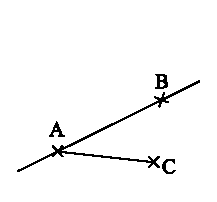
\includegraphics[width=.2\linewidth]{tracerAB-AC} & 
   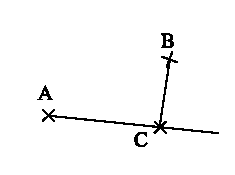
\includegraphics[width=.2\linewidth]{tracerAC-BC} & & 
   
\includegraphics[width=.2\linewidth]{tracerAB-BC-AC}& 
   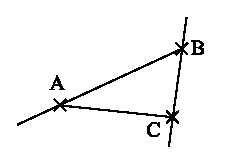
\includegraphics[width=.2\linewidth]{tracer} 					\\ \cline{1-2}\cline{4-5}
  \end{tabular}\\[1em]

  
   \item Lire la consigne de la case \circled{5} et observer la figure correspondant à cette consigne. Tracer ensuite la figure de la case \circled{6} et écrire la consigne de la case \circled{7}.
   
   \vspace{1em}
  
    \begin{tabular}{|l|l|l|}
   \hline
    \hfill \circled{5} \hfill			&	\hfill \circled{6} \hfill				&	\hfill \circled{7} \hfill 	\\
    - Tracer la droite passant par 	&	- Tracer le segment 				&					\\
    $E$ et $F$ ;					&	d'extrémités $R$ et $S$ ;			&					\\
    - Tracer le segment 			&	- Tracer la droite passant par 		&					\\
    d'extrémités $E$ et $G$ ;		&	$R$ et $T$ ;					&					\\
    - Tracer la demi-droite 			&	- Tracer la demi-droite 			&					\\
    d'origine $G$ et passant par $F$.	&	d'origine $S$ et passant par $T$.	&					\\ \hline
    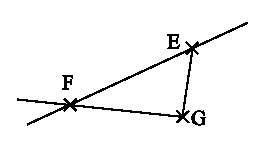
\includegraphics[width=.24\linewidth]{tracerEFG} 			&  
    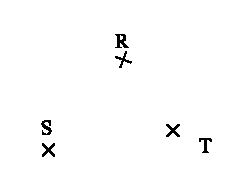
\includegraphics[width=.24\linewidth]{tracerRST}			&
    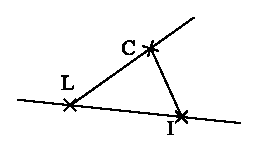
\includegraphics[width=.24\linewidth]{tracerLCI}			\\ \hline
    \end{tabular}\\[1em]

    
  \newpage
  
   \item Compléter le tableau suivant :
   
   \vspace{1em}
   
   \renewcommand*\tabularxcolumn[1]{>{\centering\arraybackslash}m{#1}}
   \begin{ttableau}{\linewidth}{3}
    \hline
    \multicolumn{1}{|c|}{\textbf{Phrase}}	&	\multicolumn{1}{c}{\textbf{Phrase codée}}	&	\multicolumn{1}{|c|}{\textbf{Dessin}}			 	\\  \hline
    								&	Tracer $[UV]$							&	
\includegraphics[width=2.6cm]{phraseUV}		\\  \hline
    								&										&	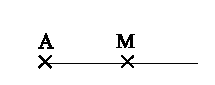
\includegraphics[width=3.2cm]{phraseAM}		\\  \hline
   Tracer la droite passant par $S$ et $T$	&										&	
\includegraphics[width=2.6cm]{phraseST}		\\  \hline
   								&										&	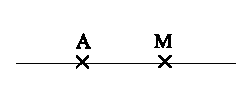
\includegraphics[width=4.0cm]{phraseAM_2}	\\  \hline
   Tracer le segment d'extrémités $M$ et $N$	&									&	
\includegraphics[width=2.6cm]{phraseMN} 	\\  \hline
   								&	Tracer $[KJ)$							&	
\includegraphics[width=2.6cm]{phraseKJ}		\\  \hline
								&										&	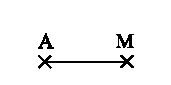
\includegraphics[width=2.6cm]{phraseAM_3}	\\  \hline
   Tracer la demi-droite d'origine $O$ et 	&										&	
\includegraphics[width=2.6cm]{phraseOU}		\\
   passant par $U$					&										&										\\  \hline
   								&	Tracer $(BC)$							&	
\includegraphics[width=2.6cm]{phraseBC}		\\  \hline
  \end{ttableau}
  
   \end{enumerate} 

\end{activite}
%%%%%%%%%%%%%%%%%%%%%%%%%%%%%%%%%%%%%%%%%%%%%


\cours
\section{Constructions graphiques : parallèles et perpendiculaires}

\begin{methode*1}[Construire la perpendiculaire à une droite passant par un point]

\begin{exemple*1}
Trace une droite $d$ et place un point $M$ n'appartenant pas à la droite $d$.

Trace la droite $d'$ perpendiculaire à la droite $d$ passant par le point $M$. \\[0.75em]

\begin{tabularx}{\textwidth}{X|X|X|X}
%manuel 6e, chapitre G3
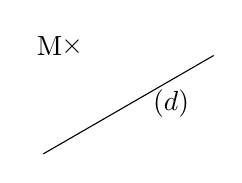
\begin{tikzpicture}[scale=0.5,every node/.style={scale=1},rotate=30]

\draw (0,2) node [left]{M};
\draw (0,2) node {$\times$};
\draw (-2,0)--(3,0) node [near end,below] {$(d)$};


\end{tikzpicture} 
 &  %manuel 6e, chapitre G3
\begin{tikzpicture}[scale=0.5,every node/.style={scale=1},rotate=30]

\draw (0,2) node [left]{M};
\draw (0,2) node {$\times$};
\draw (-2,0)--(3,0) node [near end,below] {$(d)$};
\draw [thick](-0.02,4.2)--(-0.02,2.45);

%%%%%%%%%%%%%%%%%%%%%%%%
%%%%%%%%%%%%%%%%%%%%%%%%
%Définition des paramètres de l'équerre
%et de son positionnement
%%%%%%%%%%%%%%%%%%%%%%%%
%%%%%%%%%%%%%%%%%%%%%%%%

\def \xorigine {0}; %abscisse de l'origine de l'équerre posée avec un xshift
\def \yorigine {0}; %ordonnée de l'origine de l'équerre posée avec un yshift
\def \rotation {0}; %angle de rotation de l'équerre
\def \longueur {4}; %longueur de l'équerre
\def \largeur {2}; %largeur de l'équerre
\def \epaisseur {\longueur * 0.1}; %épaisseur de la partie «colorée» de l'équerre

%%%%%%%%%%%%%%%%%%%%%%%%
%%%%%%%%%%%%%%%%%%%%%%%%
%Tracé de l'équerre
%%%%%%%%%%%%%%%%%%%%%%%%
%%%%%%%%%%%%%%%%%%%%%%%%

\begin{scope}[scale=1.1,xshift=\xorigine cm,yshift=\yorigine cm,rotate=\rotation]

%contour extérieur de l'équerre
\coordinate (A) at (0,0) ; %«origine» de l'équerre
\coordinate (B) at (\largeur,0) ;
\coordinate (C) at (0,\longueur) ;
\draw [gray](A)--(B)--(C)--cycle;


%contour intérieur de l'équerre
\coordinate (D) at (\epaisseur,\epaisseur) ;
\coordinate (E) at ($\largeur*(1,0)-{\largeur * \epaisseur / \longueur}*(1,0)-\epaisseur*(1,0)+\epaisseur*(0,1)$);
\coordinate (F) at ($\epaisseur*(1,0)+\longueur*(0,1)-{2*\longueur * \epaisseur / \largeur}*(0,1)$);
\draw [gray](D)--(E)--(F)--cycle;

%partie colorée de l'équerre
\fill [color=blue!50!gray,opacity=.4,even odd rule] (A)--(B)--(C)--cycle (D)--(E)--(F)--cycle;%l'option even odd rule permet de faire le remplissage entre les 2 zones définies
\end{scope}

%%%%%%%%%%%%%%%%%%%%%%%%
%%%%%%%%%%%%%%%%%%%%%%%%
%Fin de l'équerre
%%%%%%%%%%%%%%%%%%%%%%%%
%%%%%%%%%%%%%%%%%%%%%%%%


%%%%%%%%%%%%%%%%%%%%%%%%
%%%%%%%%%%%%%%%%%%%%%%%%
%Début crayon
%%%%%%%%%%%%%%%%%%%%%%%%
%%%%%%%%%%%%%%%%%%%%%%%%

\begin{scope}[scale=0.35,xshift=0cm,yshift=7cm,rotate=-70] %le crayon, xshift et yshift pour les coordonnées de la pointe, rotate pour l'orientation du crayon
\def \couleur {black}
\coordinate (O) at (0,0);
\fill[\couleur!40] (-0.2,4.8) -- (0.2,4.8) -- (0.2,0.8) --(0.1,0.65) -- (0,0.8) -- (-0.1,0.66) -- (-0.2,0.8) -- cycle; %corps du crayon
\draw[color=white] (0,4.8) -- (0,0.8); %trait intérieur du crayon
\fill[\couleur!90] (-0.2,4.3) -- (0,4.27) -- (0.2,4.3) -- (0.2,4.8) arc(30:150:0.23cm); %partie haute du crayon
\fill[brown!40] (-0.2,0.8) -- (O)node[coordinate,pos=0.75](a){} -- (0.2,0.8)node[coordinate,pos=0.25](b){} -- (0.1,0.65) -- (0,0.8) -- (-0.1,0.66) -- cycle; %pointe du crayon (partie taillée)
\fill[\couleur!90] (a) -- (O) -- (b) -- cycle; %mine du crayon
\end{scope}

%%%%%%%%%%%%%%%%%%%%%%%%
%%%%%%%%%%%%%%%%%%%%%%%%
%Fin crayon
%%%%%%%%%%%%%%%%%%%%%%%%
%%%%%%%%%%%%%%%%%%%%%%%%


\end{tikzpicture} 
 & %manuel 6e, chapitre G3
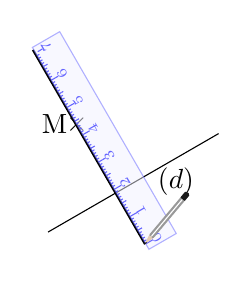
\begin{tikzpicture}[scale=0.5,every node/.style={scale=1},rotate=30]

\draw (0,2) node [left]{M};
\draw (0,2) node {$\times$};
\draw (-2,0)--(3,0) node [near end,below] {$(d)$};
\draw [thick](-0.02,4.2)--(-0.02,-1.5);

%%%%%%%%%%%%%%%%%%%%%%%%
%%%%%%%%%%%%%%%%%%%%%%%%
%Début règle
%%%%%%%%%%%%%%%%%%%%%%%%
%%%%%%%%%%%%%%%%%%%%%%%% 

    %Graduaton max. de la règle
    \def \Taille {7}
    %Définition de l 'angle de rotation de la règle
    \def \Rotation {90}
    %Définition du décalage de la règle
    \def \DecalX {0.4}
    \def \DecalY {-1.5}
    %Couleur des élèments de la règle (sauf le remplissage)
    \def \RegleColor {blue!60}

\begin{scope}[shift={(\DecalX,\DecalY)},rotate=\Rotation,scale=0.8]
    % contours de la règle
    \draw[color=\RegleColor, fill =blue!5, opacity=0.5] (-0.2,0.5) rectangle (\Taille+0.2,-0.5);	%Dont couleur de remplissage
    % graduation 1 mm
    \foreach \a in {0,0.1,...,\Taille}{\draw[color=\RegleColor] (\a,0.5)--(\a,0.42);}
    % graduation 5 mm
    \foreach \a in {0,0.5,...,\Taille}{\draw[color=\RegleColor] (\a,0.42)--(\a,0.35);}
    % graduation et repères 10 mm
    \foreach \a in {0,1,...,\Taille}{\draw[color=\RegleColor] (\a,0.35)--(\a,0.25)
    node[font=\tiny, rotate=\Rotation+30] (\a) at (\a,0.1){\a};}
\end{scope}

%%%%%%%%%%%%%%%%%%%%%%%%
%%%%%%%%%%%%%%%%%%%%%%%%
%Fin de la règle
%%%%%%%%%%%%%%%%%%%%%%%%
%%%%%%%%%%%%%%%%%%%%%%%%

%%%%%%%%%%%%%%%%%%%%%%%%
%%%%%%%%%%%%%%%%%%%%%%%%
%Début crayon
%%%%%%%%%%%%%%%%%%%%%%%%
%%%%%%%%%%%%%%%%%%%%%%%%

\begin{scope}[scale=0.35,xshift=-0.1cm,yshift=-4.28cm,rotate=-70] %le crayon, xshift et yshift pour les coordonnées de la pointe, rotate pour l'orientation du crayon
\def \couleur {black}
\coordinate (O) at (0,0);
\fill[\couleur!40] (-0.2,4.8) -- (0.2,4.8) -- (0.2,0.8) --(0.1,0.65) -- (0,0.8) -- (-0.1,0.66) -- (-0.2,0.8) -- cycle; %corps du crayon
\draw[color=white] (0,4.8) -- (0,0.8); %trait intérieur du crayon
\fill[\couleur!90] (-0.2,4.3) -- (0,4.27) -- (0.2,4.3) -- (0.2,4.8) arc(30:150:0.23cm); %partie haute du crayon
\fill[brown!40] (-0.2,0.8) -- (O)node[coordinate,pos=0.75](a){} -- (0.2,0.8)node[coordinate,pos=0.25](b){} -- (0.1,0.65) -- (0,0.8) -- (-0.1,0.66) -- cycle; %pointe du crayon (partie taillée)
\fill[\couleur!90] (a) -- (O) -- (b) -- cycle; %mine du crayon
\end{scope}

%%%%%%%%%%%%%%%%%%%%%%%%
%%%%%%%%%%%%%%%%%%%%%%%%
%Fin crayon
%%%%%%%%%%%%%%%%%%%%%%%%
%%%%%%%%%%%%%%%%%%%%%%%%


\end{tikzpicture} 
  &  %manuel 6e, chapitre G3
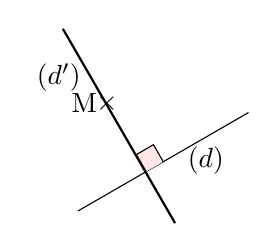
\begin{tikzpicture}[scale=0.5,every node/.style={scale=1},rotate=30]

\draw (0,2) node [left]{M};
\draw (0,2) node {$\times$};
\draw (-2,0)--(3,0) node [near end,below] {$(d)$};
\draw [thick](-0.02,4.2)--(-0.02,-1.5) node[near start,left]{$(d')$};
\draw [fill=pink!40!white](0,0)--(0,0.5)--(0.5,0.5)--(0.5,0);

\end{tikzpicture} 
 \\ 
 On trace une droite $d$ et on place un point $M$. & On place l'un des côtés de l'angle droit de l'équerre sur la droite $d$ et l'autre côté sur $M$.
 & On prolonge la droite à la règle. & On nomme la droite $d'$ et on code l'angle droit par un carré.\\

\end{tabularx} \\
 
 \end{exemple*1}


\exercice

En utilisant cette méthode, tracer un rectangle ABCD de longueur 3 cm et de longueur 5 cm.

%\correction

 
\end{methode*1}

\newpage

%%%%%%%%%%%%%%%%%%%%%%%%%%%%%

\begin{methode*1}[Construire la parallèle à une droite passant par un point]

\begin{exemple*1}
Trace une droite $d$ et place un point $M$ n'appartenant pas à la droite $d$.

Trace la droite $d'$ parallèle à la droite $d$ passant par le point $M$. \\[0.75em]

\begin{tabularx}{1.15\textwidth}{X|X|X|X}
%manuel 6e, chapitre G3
\begin{tikzpicture}[scale=.5,every node/.style={scale=1},rotate=30]

\draw (0,2) node [above left]{M};
\draw (0,2) node {$\times$};
\draw (-2.2,0)--(2.6,0) node [near end,below] {$(d)$};


%%%%%%%%%%%%%%%%%%%%%%%%
%%%%%%%%%%%%%%%%%%%%%%%%
%Définition des paramètres de l'équerre
%et de son positionnement
%%%%%%%%%%%%%%%%%%%%%%%%
%%%%%%%%%%%%%%%%%%%%%%%%

\def \xorigine {-1.65}; %abscisse de l'origine de l'équerre posée avec un xshift
\def \yorigine {0}; %ordonnée de l'origine de l'équerre posée avec un yshift
\def \rotation {-90}; %angle de rotation de l'équerre
\def \longueur {4}; %longueur de l'équerre
\def \largeur {2}; %largeur de l'équerre
\def \epaisseur {\longueur * 0.1}; %épaisseur de la partie «colorée» de l'équerre

%%%%%%%%%%%%%%%%%%%%%%%%
%%%%%%%%%%%%%%%%%%%%%%%%
%Tracé de l'équerre
%%%%%%%%%%%%%%%%%%%%%%%%
%%%%%%%%%%%%%%%%%%%%%%%%

\begin{scope}[scale=.6,xshift=\xorigine cm,yshift=\yorigine cm,rotate=\rotation]

%contour extérieur de l'équerre
\coordinate (A) at (0,0) ; %«origine» de l'équerre
\coordinate (B) at (\largeur,0) ;
\coordinate (C) at (0,\longueur) ;
\draw [gray](A)--(B)--(C)--cycle;


%contour intérieur de l'équerre
\coordinate (D) at (\epaisseur,\epaisseur) ;
\coordinate (E) at ($\largeur*(1,0)-{\largeur * \epaisseur / \longueur}*(1,0)-\epaisseur*(1,0)+\epaisseur*(0,1)$);
\coordinate (F) at ($\epaisseur*(1,0)+\longueur*(0,1)-{2*\longueur * \epaisseur / \largeur}*(0,1)$);
\draw [gray](D)--(E)--(F)--cycle;

%partie colorée de l'équerre
\fill [color=blue!50!gray,opacity=.4,even odd rule] (A)--(B)--(C)--cycle (D)--(E)--(F)--cycle;%l'option even odd rule permet de faire le remplissage entre les 2 zones définies

\end{scope}
%%%%%%%%%%%%%%%%%%%%%%%%
%%%%%%%%%%%%%%%%%%%%%%%%
%Fin de l'équerre
%%%%%%%%%%%%%%%%%%%%%%%%
%%%%%%%%%%%%%%%%%%%%%%%%


\end{tikzpicture} 
  &  %manuel 6e, chapitre G3
\begin{tikzpicture}[scale=.5,every node/.style={scale=1},rotate=30]

\draw (0,2) node [above left]{M};
\draw (0,2) node {$\times$};
\draw (-2.2,0)--(2.6,0) node [near end,below] {$(d)$};


%%%%%%%%%%%%%%%%%%%%%%%%
%%%%%%%%%%%%%%%%%%%%%%%%
%Définition des paramètres de l'équerre
%et de son positionnement
%%%%%%%%%%%%%%%%%%%%%%%%
%%%%%%%%%%%%%%%%%%%%%%%%

\def \xorigine {-1.65}; %abscisse de l'origine de l'équerre posée avec un xshift
\def \yorigine {0}; %ordonnée de l'origine de l'équerre posée avec un yshift
\def \rotation {-90}; %angle de rotation de l'équerre
\def \longueur {4}; %longueur de l'équerre
\def \largeur {2}; %largeur de l'équerre
\def \epaisseur {\longueur * 0.1}; %épaisseur de la partie «colorée» de l'équerre

%%%%%%%%%%%%%%%%%%%%%%%%
%%%%%%%%%%%%%%%%%%%%%%%%
%Tracé de l'équerre
%%%%%%%%%%%%%%%%%%%%%%%%
%%%%%%%%%%%%%%%%%%%%%%%%

\begin{scope}[scale=.6,xshift=\xorigine cm,yshift=\yorigine cm,rotate=\rotation]

%contour extérieur de l'équerre
\coordinate (A) at (0,0) ; %«origine» de l'équerre
\coordinate (B) at (\largeur,0) ;
\coordinate (C) at (0,\longueur) ;
\draw [gray](A)--(B)--(C)--cycle;


%contour intérieur de l'équerre
\coordinate (D) at (\epaisseur,\epaisseur) ;
\coordinate (E) at ($\largeur*(1,0)-{\largeur * \epaisseur / \longueur}*(1,0)-\epaisseur*(1,0)+\epaisseur*(0,1)$);
\coordinate (F) at ($\epaisseur*(1,0)+\longueur*(0,1)-{2*\longueur * \epaisseur / \largeur}*(0,1)$);
\draw [gray](D)--(E)--(F)--cycle;

%partie colorée de l'équerre
\fill [color=blue!50!gray,opacity=.4,even odd rule] (A)--(B)--(C)--cycle (D)--(E)--(F)--cycle;%l'option even odd rule permet de faire le remplissage entre les 2 zones définies

\end{scope}
%%%%%%%%%%%%%%%%%%%%%%%%
%%%%%%%%%%%%%%%%%%%%%%%%
%Fin de l'équerre
%%%%%%%%%%%%%%%%%%%%%%%%
%%%%%%%%%%%%%%%%%%%%%%%%

%%%%%%%%%%%%%%%%%%%%%%%%
%%%%%%%%%%%%%%%%%%%%%%%%
%Début règle !! Si la figure est tournée, il faut
%rajouter l'angle de rotation dans le node des graduation
%pour que les nombres soient écrits correctement
%%%%%%%%%%%%%%%%%%%%%%%%
%%%%%%%%%%%%%%%%%%%%%%%% 

    %Graduaton max. de la règle
    \def \Taille {5}
    %Définition de l 'angle de rotation de la règle
    \def \Rotation {-90}
    %Définition du décalage de la règle
    \def \DecalX {-1.5}
    \def \DecalY {2.8}
    %Couleur des élèments de la règle (sauf le remplissage)
    \def \RegleColor {blue!60}

\begin{scope}[shift={(\DecalX,\DecalY)},rotate=\Rotation,scale=1]
    % contours de la règle
    \draw[color=\RegleColor, fill =blue!5, opacity=0.5] (-0.2,0.5) rectangle (\Taille+0.2,-0.5);	%Dont couleur de remplissage
    % graduation 1 mm
    \foreach \a in {0,0.1,...,\Taille}{\draw[color=\RegleColor] (\a,0.5)--(\a,0.42);}
    % graduation 5 mm
    \foreach \a in {0,0.5,...,\Taille}{\draw[color=\RegleColor] (\a,0.42)--(\a,0.35);}
    % graduation et repères 10 mm
    \foreach \a in {0,1,...,\Taille}{\draw[color=\RegleColor] (\a,0.35)--(\a,0.25)
    node[font=\tiny, rotate=\Rotation+30] (\a) at (\a,0.1){\a};}%ici rajouter l'angle de rotation de la figure complète pour que les nombres soient écrits correctement
\end{scope}

%%%%%%%%%%%%%%%%%%%%%%%%
%%%%%%%%%%%%%%%%%%%%%%%%
%Fin de la règle
%%%%%%%%%%%%%%%%%%%%%%%%
%%%%%%%%%%%%%%%%%%%%%%%%


\end{tikzpicture} 
 & %manuel 6e, chapitre G3
\begin{tikzpicture}[scale=.5,every node/.style={scale=1},rotate=30]

\draw (0,2) node [above left]{M};
\draw (0,2) node {$\times$};
\draw (-2.2,0)--(2.6,0) node [near end,below] {$(d)$};
\draw [very thick,red,dashed,->,>=stealth] (-0.5,0)--(-0.5,2);


%%%%%%%%%%%%%%%%%%%%%%%%
%%%%%%%%%%%%%%%%%%%%%%%%
%Définition des paramètres de l'équerre
%et de son positionnement
%%%%%%%%%%%%%%%%%%%%%%%%
%%%%%%%%%%%%%%%%%%%%%%%%

\def \xorigine {-1.65}; %abscisse de l'origine de l'équerre posée avec un xshift
\def \yorigine {0}; %ordonnée de l'origine de l'équerre posée avec un yshift
\def \rotation {-90}; %angle de rotation de l'équerre
\def \longueur {4}; %longueur de l'équerre
\def \largeur {2}; %largeur de l'équerre
\def \epaisseur {\longueur * 0.1}; %épaisseur de la partie «colorée» de l'équerre

%%%%%%%%%%%%%%%%%%%%%%%%
%%%%%%%%%%%%%%%%%%%%%%%%
%Tracé de l'équerre
%%%%%%%%%%%%%%%%%%%%%%%%
%%%%%%%%%%%%%%%%%%%%%%%%

\begin{scope}[scale=.6,xshift=\xorigine cm,yshift=\yorigine cm,rotate=\rotation]

%contour extérieur de l'équerre
\coordinate (A) at (0,0) ; %«origine» de l'équerre
\coordinate (B) at (\largeur,0) ;
\coordinate (C) at (0,\longueur) ;
\draw [gray, opacity=0.2](A)--(B)--(C)--cycle;


%contour intérieur de l'équerre
\coordinate (D) at (\epaisseur,\epaisseur) ;
\coordinate (E) at ($\largeur*(1,0)-{\largeur * \epaisseur / \longueur}*(1,0)-\epaisseur*(1,0)+\epaisseur*(0,1)$);
\coordinate (F) at ($\epaisseur*(1,0)+\longueur*(0,1)-{2*\longueur * \epaisseur / \largeur}*(0,1)$);
\draw [gray, opacity=0.2](D)--(E)--(F)--cycle;

%partie colorée de l'équerre
\fill [color=blue!50!gray,opacity=.1,even odd rule] (A)--(B)--(C)--cycle (D)--(E)--(F)--cycle;%l'option even odd rule permet de faire le remplissage entre les 2 zones définies

\end{scope}
%%%%%%%%%%%%%%%%%%%%%%%%
%%%%%%%%%%%%%%%%%%%%%%%%
%Fin de l'équerre
%%%%%%%%%%%%%%%%%%%%%%%%
%%%%%%%%%%%%%%%%%%%%%%%%


%%%%%%%%%%%%%%%%%%%%%%%%
%%%%%%%%%%%%%%%%%%%%%%%%
%Définition des paramètres de l'équerre
%et de son positionnement
%%%%%%%%%%%%%%%%%%%%%%%%
%%%%%%%%%%%%%%%%%%%%%%%%

\def \yorigine2 {3.3}; %ordonnée de l'origine de l'équerre posée avec un yshift

%%%%%%%%%%%%%%%%%%%%%%%%
%%%%%%%%%%%%%%%%%%%%%%%%
%Tracé de l'équerre
%%%%%%%%%%%%%%%%%%%%%%%%
%%%%%%%%%%%%%%%%%%%%%%%%

\begin{scope}[scale=.6,xshift=\xorigine cm,yshift=\yorigine2 cm,rotate=\rotation]

%contour extérieur de l'équerre
\coordinate (A) at (0,0) ; %«origine» de l'équerre
\coordinate (B) at (\largeur,0) ;
\coordinate (C) at (0,\longueur) ;
\draw [gray](A)--(B)--(C)--cycle;


%contour intérieur de l'équerre
\coordinate (D) at (\epaisseur,\epaisseur) ;
\coordinate (E) at ($\largeur*(1,0)-{\largeur * \epaisseur / \longueur}*(1,0)-\epaisseur*(1,0)+\epaisseur*(0,1)$);
\coordinate (F) at ($\epaisseur*(1,0)+\longueur*(0,1)-{2*\longueur * \epaisseur / \largeur}*(0,1)$);
\draw [gray](D)--(E)--(F)--cycle;

%partie colorée de l'équerre
\fill [color=blue!50!gray,opacity=.4,even odd rule] (A)--(B)--(C)--cycle (D)--(E)--(F)--cycle;%l'option even odd rule permet de faire le remplissage entre les 2 zones définies

\end{scope}
%%%%%%%%%%%%%%%%%%%%%%%%
%%%%%%%%%%%%%%%%%%%%%%%%
%Fin de l'équerre
%%%%%%%%%%%%%%%%%%%%%%%%
%%%%%%%%%%%%%%%%%%%%%%%%



%%%%%%%%%%%%%%%%%%%%%%%%
%%%%%%%%%%%%%%%%%%%%%%%%
%Début règle !! Si la figure est tournée, il faut
%rajouter l'angle de rotation dans le node des graduation
%pour que les nombres soient écrits correctement
%%%%%%%%%%%%%%%%%%%%%%%%
%%%%%%%%%%%%%%%%%%%%%%%% 

    %Graduaton max. de la règle
    \def \Taille {5}
    %Définition de l 'angle de rotation de la règle
    \def \Rotation {-90}
    %Définition du décalage de la règle
    \def \DecalX {-1.5}
    \def \DecalY {2.8}
    %Couleur des élèments de la règle (sauf le remplissage)
    \def \RegleColor {blue!60}

\begin{scope}[shift={(\DecalX,\DecalY)},rotate=\Rotation,scale=1]
    % contours de la règle
    \draw[color=\RegleColor, fill =blue!5, opacity=0.5] (-0.2,0.5) rectangle (\Taille+0.2,-0.5);	%Dont couleur de remplissage
    % graduation 1 mm
    \foreach \a in {0,0.1,...,\Taille}{\draw[color=\RegleColor] (\a,0.5)--(\a,0.42);}
    % graduation 5 mm
    \foreach \a in {0,0.5,...,\Taille}{\draw[color=\RegleColor] (\a,0.42)--(\a,0.35);}
    % graduation et repères 10 mm
    \foreach \a in {0,1,...,\Taille}{\draw[color=\RegleColor] (\a,0.35)--(\a,0.25)
    node[font=\tiny, rotate=\Rotation+30] (\a) at (\a,0.1){\a};}%ici rajouter l'angle de rotation de la figure complète pour que les nombres soient écrits correctement
\end{scope}

%%%%%%%%%%%%%%%%%%%%%%%%
%%%%%%%%%%%%%%%%%%%%%%%%
%Fin de la règle
%%%%%%%%%%%%%%%%%%%%%%%%
%%%%%%%%%%%%%%%%%%%%%%%%


\end{tikzpicture} 
 &  %manuel 6e, chapitre G3
\begin{tikzpicture}[scale=.5,every node/.style={scale=1},rotate=30]

\draw (0,2) node [above left]{M};
\draw (0,2) node {$\times$};
\draw (-2.2,0)--(2.6,0) node [near end,below] {$(d)$};
\draw [red](-1,2)--(0.5,2);

%%%%%%%%%%%%%%%%%%%%%%%%
%%%%%%%%%%%%%%%%%%%%%%%%
%Définition des paramètres de l'équerre
%et de son positionnement
%%%%%%%%%%%%%%%%%%%%%%%%
%%%%%%%%%%%%%%%%%%%%%%%%

\def \xorigine {-1.65}; %abscisse de l'origine de l'équerre posée avec un xshift
\def \yorigine {0}; %ordonnée de l'origine de l'équerre posée avec un yshift
\def \rotation {-90}; %angle de rotation de l'équerre
\def \longueur {4}; %longueur de l'équerre
\def \largeur {2}; %largeur de l'équerre
\def \epaisseur {\longueur * 0.1}; %épaisseur de la partie «colorée» de l'équerre
\def \yorigine2 {3.31}; %ordonnée de l'origine de l'équerre posée avec un yshift

%%%%%%%%%%%%%%%%%%%%%%%%
%%%%%%%%%%%%%%%%%%%%%%%%
%Tracé de l'équerre
%%%%%%%%%%%%%%%%%%%%%%%%
%%%%%%%%%%%%%%%%%%%%%%%%

\begin{scope}[scale=.6,xshift=\xorigine cm,yshift=\yorigine2 cm,rotate=\rotation]

%contour extérieur de l'équerre
\coordinate (A) at (0,0) ; %«origine» de l'équerre
\coordinate (B) at (\largeur,0) ;
\coordinate (C) at (0,\longueur) ;
\draw [gray](A)--(B)--(C)--cycle;


%contour intérieur de l'équerre
\coordinate (D) at (\epaisseur,\epaisseur) ;
\coordinate (E) at ($\largeur*(1,0)-{\largeur * \epaisseur / \longueur}*(1,0)-\epaisseur*(1,0)+\epaisseur*(0,1)$);
\coordinate (F) at ($\epaisseur*(1,0)+\longueur*(0,1)-{2*\longueur * \epaisseur / \largeur}*(0,1)$);
\draw [gray](D)--(E)--(F)--cycle;

%partie colorée de l'équerre
\fill [color=blue!50!gray,opacity=.4,even odd rule] (A)--(B)--(C)--cycle (D)--(E)--(F)--cycle;%l'option even odd rule permet de faire le remplissage entre les 2 zones définies

\end{scope}
%%%%%%%%%%%%%%%%%%%%%%%%
%%%%%%%%%%%%%%%%%%%%%%%%
%Fin de l'équerre
%%%%%%%%%%%%%%%%%%%%%%%%
%%%%%%%%%%%%%%%%%%%%%%%%



%%%%%%%%%%%%%%%%%%%%%%%%
%%%%%%%%%%%%%%%%%%%%%%%%
%Début règle !! Si la figure est tournée, il faut
%rajouter l'angle de rotation dans le node des graduation
%pour que les nombres soient écrits correctement
%%%%%%%%%%%%%%%%%%%%%%%%
%%%%%%%%%%%%%%%%%%%%%%%% 

    %Graduaton max. de la règle
    \def \Taille {5}
    %Définition de l 'angle de rotation de la règle
    \def \Rotation {-90}
    %Définition du décalage de la règle
    \def \DecalX {-1.5}
    \def \DecalY {2.8}
    %Couleur des élèments de la règle (sauf le remplissage)
    \def \RegleColor {blue!60}

\begin{scope}[shift={(\DecalX,\DecalY)},rotate=\Rotation,scale=1]
    % contours de la règle
    \draw[color=\RegleColor, fill =blue!5, opacity=0.5] (-0.2,0.5) rectangle (\Taille+0.2,-0.5);	%Dont couleur de remplissage
    % graduation 1 mm
    \foreach \a in {0,0.1,...,\Taille}{\draw[color=\RegleColor] (\a,0.5)--(\a,0.42);}
    % graduation 5 mm
    \foreach \a in {0,0.5,...,\Taille}{\draw[color=\RegleColor] (\a,0.42)--(\a,0.35);}
    % graduation et repères 10 mm
    \foreach \a in {0,1,...,\Taille}{\draw[color=\RegleColor] (\a,0.35)--(\a,0.25)
    node[font=\tiny, rotate=\Rotation+30] (\a) at (\a,0.1){\a};}%ici rajouter l'angle de rotation de la figure complète pour que les nombres soient écrits correctement
\end{scope}

%%%%%%%%%%%%%%%%%%%%%%%%
%%%%%%%%%%%%%%%%%%%%%%%%
%Fin de la règle
%%%%%%%%%%%%%%%%%%%%%%%%
%%%%%%%%%%%%%%%%%%%%%%%%

%%%%%%%%%%%%%%%%%%%%%%%%
%%%%%%%%%%%%%%%%%%%%%%%%
%Début crayon
%%%%%%%%%%%%%%%%%%%%%%%%
%%%%%%%%%%%%%%%%%%%%%%%%

\begin{scope}[scale=0.3,xshift=1.65cm,yshift=6.65cm,rotate=-70] %le crayon, xshift et yshift pour les coordonnées de la pointe, rotate pour l'orientation du crayon
\def \couleur {black}
\coordinate (O) at (0,0);
\fill[\couleur!40] (-0.2,4.8) -- (0.2,4.8) -- (0.2,0.8) --(0.1,0.65) -- (0,0.8) -- (-0.1,0.66) -- (-0.2,0.8) -- cycle; %corps du crayon
\draw[color=white] (0,4.8) -- (0,0.8); %trait intérieur du crayon
\fill[red] (-0.2,4.3) -- (0,4.27) -- (0.2,4.3) -- (0.2,4.8) arc(30:150:0.23cm); %partie haute du crayon
\fill[brown!40] (-0.2,0.8) -- (O)node[coordinate,pos=0.75](a){} -- (0.2,0.8)node[coordinate,pos=0.25](b){} -- (0.1,0.65) -- (0,0.8) -- (-0.1,0.66) -- cycle; %pointe du crayon (partie taillée)
\fill[red] (a) -- (O) -- (b) -- cycle; %mine du crayon
\end{scope}

%%%%%%%%%%%%%%%%%%%%%%%%
%%%%%%%%%%%%%%%%%%%%%%%%
%Fin crayon
%%%%%%%%%%%%%%%%%%%%%%%%
%%%%%%%%%%%%%%%%%%%%%%%%


\end{tikzpicture} 
\\ 
On trace une droite $d$, on place un point $M$. On place l'un des côtés de l'angle droit de l'équerre sur la droite $d$. & On place la règle le long de l'autre côté de l'équerre & On tient bien la règle et on fait coulisser l'équerre le long de la règle, jusqu'au point $M$. & On trace ainsi la droite $d'$ et on obtient :\vspace{0.3em}
%manuel 6e, chapitre G3
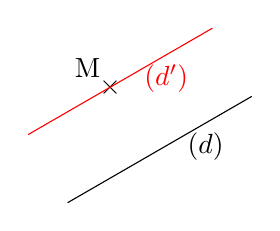
\begin{tikzpicture}[scale=.5,every node/.style={scale=1},rotate=30]

\draw (0,2) node [above left]{M};
\draw (0,2) node {$\times$};
\draw (-2.4,0)--(3,0) node [near end,below] {$(d)$};
\draw [red](-2.4,2)--(3,2) node [near end,below] {$(d')$};

\end{tikzpicture} 
\\
\end{tabularx} \\
 \end{exemple*1}

\exercice

Trace dans ton cahier un segment $[AB]$ d'une longueur de 5 cm et place un point $C$ au-dessus du segment $[AB]$ ($C$ n'est pas sur le segment). Construis, en rouge, la perpendiculaire à $[AB]$ passant par $C$. Construis, en vert, la parallèle à $[AB]$ passant par $C$.
%\correction

\end{methode*1}

\begin{aconnaitre}
\textbf{\underline{Propriété:}}\\
Si deux droites sont parallèles et si une troisième droite est perpendiculaire à l'une d'elle, alors elles est perpendiculaire à l'autre.
\end{aconnaitre}

\begin{methode*1}[Illustration]
\begin{exemple*1}

Soit $(d)$ et $(d')$ deux droites parallèles. Soit $(\Delta)$ un troisième droite.\\
Si $(d)$ et $(\Delta)$ sont perpendiculaires alors $(d')$ et $(\Delta)$ sont également perpendicualires.

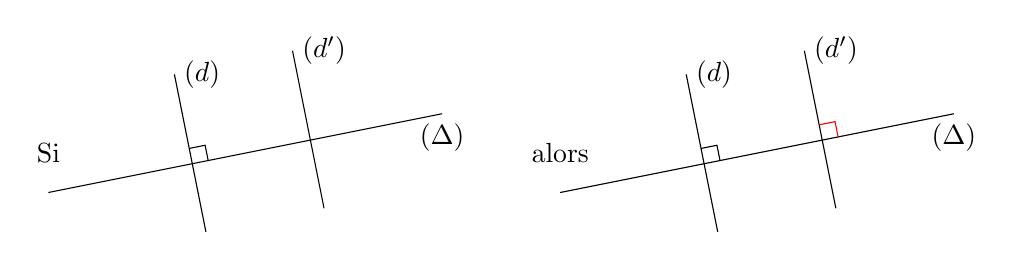
\begin{tikzpicture}
\draw (-2.0,0) node {Si} (-2,-0.5) -- ++(5,1) node[below] {$(\Delta)$} ;
%\draw (-2.0,0) node {Si} (-2,-0.5) ++(1,0.2) -- ++(4,0.8) node[below] {$(\Delta)$} ;
\draw (0,-1) -- ++(-0.4,2) node[right] {$(d)$};
\draw (1.5,-0.7) -- ++(-0.4,2) node[right] {$(d^\prime)$};
\draw (-0.17,-0.14) ++(0.2,0.04) -- ++(-0.04,0.2) -- ++(-0.2, -0.04); %circle (1pt);


\draw (4.5,0) node {alors} ++(0,-0.5) -- ++(5,1) node[below] {$(\Delta)$} ;
\draw (6.5,-1) -- ++(-0.4,2) node[right] {$(d)$};
\draw (8.0,-0.7) -- ++(-0.4,2) node[right] {$(d^\prime)$};
\draw (6.33,-0.14) ++(0.2,0.04) -- ++(-0.04,0.2) -- ++(-0.2, -0.04);
\draw[red] (7.83,0.16) ++(0.2,0.04) -- ++(-0.04,0.2) -- ++(-0.2, -0.04); %circle (1pt);

\end{tikzpicture}
\end{exemple*1}

\exercice

Dans la figure ci-contre:\
\begin{itemize}
\item Tracer la droite $(AB)$.
\item Construire la droite $(d)$ parallèle à $(AB)$ passant par $C$.
\item Construire la droite $(d')$ perpendiculaire à $(AB)$ passant par $B$.
\item Que peut-on dire des droites $(d)$ et $(d')$? Justifier.\\
\end{itemize}
\begin{center}
\tikzset{
   cross/.pic = {
     \draw[thick] (-0.2,0.2) -- (0.2,-0.2);
     \draw[thick] (-0.2,-0.2) -- (0.2,0.2);}
}


\begin{tikzpicture}
\draw (0,0) rectangle (10,6);
\pic[scale=0.6] at (1,3) {cross}; \draw (1,3.5) node {\large $A$};
\pic[scale=0.6] at (6,5) {cross}; \draw (6,5.5) node {\large $B$};
\pic[scale=0.6] at (9,2) {cross}; \draw (9,2.5) node {\large $C$};
\end{tikzpicture}
\end{center}
\end{methode*1}


%%%%%%%%%%%%%%%%%%%%%%%%%%%%%
\newpage

\section{La médiatrice}

\begin{definition}
La \textbf{\MotDefinition{médiatrice}{}} d'un segment est la droite qui coupe ce segment perpendiculairement en son milieu.
\end{definition}


\begin{methode*1}[Construire une médiatrice]

\begin{exemple*1}
Trace un segment $[OS]$ de longueur 5 cm puis sa médiatrice. \\[0.75em]

\begin{tabularx}{\textwidth}{X|X|X|X}
%manuel 6e, chapitre G3

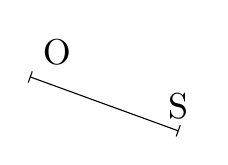
\begin{tikzpicture}[scale=0.5,every node/.style={scale=1.3}]

\def \CharSize {2.5};

\begin{scope}[rotate=-20]
\draw (-2,0)--(2,0);
\draw (-2,0)--+(90:0.15)--+(-90:0.15);
\draw (2,0)--+(90:0.15)--+(-90:0.15);
\node [above right] at (-2,0) {O};
\node [above] at (2,0) {S};
\end{scope}

\end{tikzpicture}  &

% Attention, il faut déclarer la librairie calc :\usetikzlibrary{calc}  pour les calculs de coordonnées des points


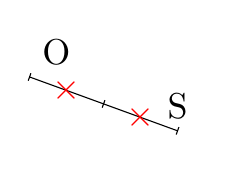
\begin{tikzpicture}	[scale=0.5,every node/.style={scale=1.3}]

\begin{scope}[rotate=-20] %la figure
\draw (-2,0)--(0,0) node [midway,red] {$\times$};
\draw (0,0)--(2,0) node [midway,red] {$\times$};
\draw (-2,0)--+(90:0.1)--+(-90:0.1);
\draw (2,0)--+(90:0.1)--+(-90:0.1);
\draw (0,0)--+(90:0.1)--+(-90:0.1);
\node [above right] at (-2,0) {O};
\node [above] at (2,0) {S};
\end{scope}

\end{tikzpicture} 
 
 & 
% Attention, il faut déclarer la librairie calc :\usetikzlibrary{calc}  pour les calculs de coordonnées des points

\begin{tikzpicture}[scale=0.5,every node/.style={scale=1.3}]
  
%%%%%%%%%%%%%%%%%%%%%%%%
%%%%%%%%%%%%%%%%%%%%%%%%
%Définition des paramètres de l'équerre
%et de son positionnement
%%%%%%%%%%%%%%%%%%%%%%%%
%%%%%%%%%%%%%%%%%%%%%%%%

\def \xorigine {0}; %abscisse de l'origine de l'équerre posée avec un xshift
\def \yorigine {0}; %ordonnée de l'origine de l'équerre posée avec un yshift
\def \rotation {-20}; %angle de rotation de l'équerre
\def \longueur {4}; %longueur de l'équerre
\def \largeur {2}; %largeur de l'équerre
\def \epaisseur {\longueur * 0.1}; %épaisseur de la partie «colorée» de l'équerre

%%%%%%%%%%%%%%%%%%%%%%%%
%%%%%%%%%%%%%%%%%%%%%%%%
%Tracé de l'équerre
%%%%%%%%%%%%%%%%%%%%%%%%
%%%%%%%%%%%%%%%%%%%%%%%%
\begin{scope}[scale=0.8,xshift=\xorigine cm,yshift=\yorigine cm,rotate=\rotation]

%contour extérieur de l'équerre
\coordinate (A) at (0,0) ; %«origine» de l'équerre
\coordinate (B) at (\largeur,0) ;
\coordinate (C) at (0,\longueur) ;
\draw [gray](A)--(B)--(C)--cycle;


%contour intérieur de l'équerre
\coordinate (D) at (\epaisseur,\epaisseur) ;
\coordinate (E) at ($\largeur*(1,0)-{\largeur * \epaisseur / \longueur}*(1,0)-\epaisseur*(1,0)+\epaisseur*(0,1)$);
\coordinate (F) at ($\epaisseur*(1,0)+\longueur*(0,1)-{2*\longueur * \epaisseur / \largeur}*(0,1)$);
\draw [gray](D)--(E)--(F)--cycle;

%partie colorée de l'équerre
\fill [color=blue!50!gray,opacity=0.5,even odd rule] (A)--(B)--(C)--cycle (D)--(E)--(F)--cycle;%l'option even odd rule permet de faire le remplissage entre les 2 zones définies

\end{scope}

\begin{scope}[scale=0.5,xshift=.32cm,yshift=3cm,rotate=30] %le crayon
\fill[gray!50] (0,4) -- (0.4,4) -- (0.4,0) --(0.3,-0.15) -- (0.2,0) -- (0.1,-0.14) -- (0,0) -- cycle;
\draw[color=white] (0.2,4) -- (0.2,0);
\fill[black] (0,3.5) -- (0.2,3.47) -- (0.4,3.5) -- (0.4,4) arc(30:150:0.23cm);
\fill[brown!40] (0,0) -- (0.2,-0.8)node[coordinate,pos=0.75](a){} --(0.4,0) node[coordinate,pos=0.25](b){} -- (0.3,-0.15) -- (0.2,0) -- (0.1,-0.14) -- cycle;
\fill[black] (a) -- (0.2,-0.8) -- (b) -- cycle;
\end{scope}

\begin{scope}[rotate=-20] %la figure
\draw (-2,0)--(0,0) node [midway,red] {$\times$};
\draw (0,0)--(2,0) node [midway,red] {$\times$};
\draw (-2,0)--+(90:0.1)--+(-90:0.1);
\draw (2,0)--+(90:0.1)--+(-90:0.1);
\draw (0,0)--+(90:0.1)--+(-90:0.1);
\node [above right] at (-2,0) {O};
\node [above] at (2,0) {S};

\draw (0,0)--($(0,0)!1.3cm!90:(2,0)$); %trace un segment de 1.3cm à 90° du segment allant de (0,0) à (2,0)

\end{scope}



\end{tikzpicture} 
  &  
% Attention, il faut déclarer la librairie calc :\usetikzlibrary{calc}  pour les calculs de coordonnées des points

\begin{tikzpicture}[scale=0.5,every node/.style={scale=1.3}]

\begin{scope}[rotate=-20] %la figure
\draw (-2,0)--(0,0) node [midway,red] {$\times$};
\draw (0,0)--(2,0) node [midway,red] {$\times$};
\draw (-2,0)--+(90:0.1)--+(-90:0.1);
\draw (2,0)--+(90:0.1)--+(-90:0.1);
\draw (0,0)--+(90:0.1)--+(-90:0.1);
\node [above right] at (-2,0) {O};
\node [above] at (2,0) {S};

\draw (0,0)--($(0,0)!2.5cm!90:(2,0)$);
\draw (0,0)--($(0,0)!1.5cm!-90:(2,0)$);
\draw (0,0)--(0.3,0)--(0.3,0.3)-|cycle;

\end{scope}



\end{tikzpicture} 
  \\ 
On trace un segment $[OS]$. & On trace le milieu du segment. & On trace la droite perpendiculaire au segment qui passe par ce milieu. & On code l'angle droit par un carré. \\
\end{tabularx} \\

 \end{exemple*1}
 
 \begin{exemple*1}
Trace un segment $[AB]$ de longueur 6 cm. Construis sa médiatrice au compas. \\[0.75em]

\begin{tabular}{l|l|l|l}
 \textcolor{H1}{\circled{1}} &  \textcolor{H1}{\circled{2}} &  \textcolor{H1}{\circled{3}} & \textcolor{H1}{\circled{1}} On trace le segment $[AB]$. \\ 
 \multirow{7}{*}{

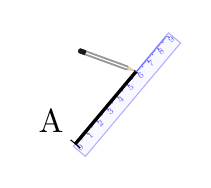
\begin{tikzpicture}[scale=0.2,rotate=50,every node/.style={scale=1.2}]

%début de la règle
    %Graduaton max. de la règle
    \def \Taille {9}
    %Définition de l 'angle de rotation de la règle
    \def \Rotation {0}
    %Définition du décalage de la règle
    \def \DecalX {0}
    \def \DecalY {0}
    %Couleur des élèments de la règle (sauf le remplissage)
    \def \RegleColor {blue!60}

\begin{scope}[scale=1,shift={(\DecalX,\DecalY)},rotate=\Rotation]
    % contours de la règle
    \draw[color=\RegleColor, fill =blue!5, opacity=0.5] (-0.2,0.5) rectangle (\Taille+0.2,-0.5);	%Dont couleur de remplissage
    % graduation 1 mm
    \foreach \a in {0,0.1,...,\Taille}{\draw[color=\RegleColor] (\a,0.5)--(\a,0.42);}
    % graduation 5 mm
    \foreach \a in {0,0.5,...,\Taille}{\draw[color=\RegleColor] (\a,0.42)--(\a,0.35);}
    % graduation et repères 10 mm
    \foreach \a in {0,1,...,\Taille}{\draw[color=\RegleColor] (\a,0.35)--(\a,0.25)
    node[scale=0.5,font=\tiny, rotate=40] (\a) at (\a,0.1){\a};}
%fin de la règle

\draw (0,0.5) node[above left]{A};
\draw (0,0.5)--+(90:0.4)--+(-90:0.4);
\draw [very thick](0,0.5)--(6,0.5);

\end{scope}

\begin{scope}[scale=0.8,xshift=7.52cm,yshift=.62cm,rotate=20] %le crayon, xshift et yshift pour les coordonnées de la pointe, rotate pour l'orientation du crayon
\def \couleur {black}
\coordinate (O) at (0,0);
\fill[\couleur!40] (-0.2,4.8) -- (0.2,4.8) -- (0.2,0.8) --(0.1,0.65) -- (0,0.8) -- (-0.1,0.66) -- (-0.2,0.8) -- cycle; %corps du crayon
\draw[color=white] (0,4.8) -- (0,0.8); %trait intérieur du crayon
\fill[\couleur!90] (-0.2,4.3) -- (0,4.27) -- (0.2,4.3) -- (0.2,4.8) arc(30:150:0.23cm); %partie haute du crayon
\fill[brown!40] (-0.2,0.8) -- (O)node[coordinate,pos=0.75](a){} -- (0.2,0.8)node[coordinate,pos=0.25](b){} -- (0.1,0.65) -- (0,0.8) -- (-0.1,0.66) -- cycle; %pointe du crayon (partie taillée)
\fill[\couleur!90] (a) -- (O) -- (b) -- cycle; %mine du crayon
\end{scope}


\end{tikzpicture}


} &  \multirow{7}{*}{

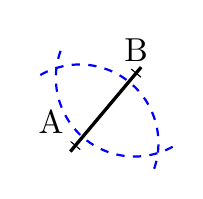
\begin{tikzpicture}[scale=0.2,rotate=50,every node/.style={scale=1.2}]

\draw [very thick](-0.5,0.5)--(6.5,0.5);
\draw (0,0.5)--+(90:0.4)--+(-90:0.4);
\draw (6,0.5)--+(90:0.4)--+(-90:0.4);
\draw (0,0.5) node[above left]{A};
\draw (6,0.5) node[above]{B};

\draw [style=dashed,color=blue,thick](4,5.083) arc (110:250:5);
\draw [style=dashed,color=blue,thick](2,5.083) arc (70:-70:5);
%\draw (3,6)--(3,-6);

\coordinate (A) at (0,0.5) ;
\coordinate (B) at (2,5.083) ;
\begin{scope}[scale=.8]
\Compas{A}{B}
\end{scope}

\end{tikzpicture}
} & \multirow{7}{*}{

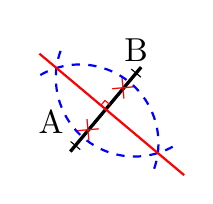
\begin{tikzpicture}[scale=0.2,rotate=50,every node/.style={scale=1.2}]

%\draw [very thick](-0.5,0.5)--(6.5,0.5);
\draw [very thick](-0.5,0.5)--(3,0.5) node[midway,red,rotate=50]{$\times$}--(6.5,0.5)node[midway,red,rotate=50]{$\times$};
\draw (0,0.5)--+(90:0.4)--+(-90:0.4);
\draw (6,0.5)--+(90:0.4)--+(-90:0.4);
\draw (0,0.5) node[above left]{A};
\draw (6,0.5) node[above]{B};

\draw [style=dashed,color=blue,thick](4,5.083) arc (110:250:5);
\draw [style=dashed,color=blue,thick](2,5.083) arc (70:-70:5);
\draw [thick,color=red](3,6)--(3,-6);
\draw [color=red](3,0.9)-|(3.4,0.5);

\end{tikzpicture}
} &  \textcolor{H1}{\circled{2}} On trace deux arcs de cercle\\ % exemple de fusion de cellules d'une même colonne
&&& de centres $A$ et $B$, de même\\ 
&&& rayon, en choisissant un\\
&&& rayon suffisamment grand\\
&&& pour que ces arcs se coupent\\
&&&  en deux points.\\ 
&&& \textcolor{H1}{\circled{3}} La médiatrice de [AB] est \\
&&&  la droite qui passe par ces\\
&&& deux points.\\ 
\end{tabular} \\

 \end{exemple*1}

\exercice 
Trace un segment $[AB]$ de 7 cm. Trace la médiatrice du segment $[AB]$ par la méthode de ton choix.
%\correction

 
\end{methode*1}

%%%%%%%%%%%%%%%%%%%%%%%%%%%%%


\section{Les angles}

%%%%%%%%%%%%%%%%%%%%%%%%%%%%%

% remarque : pour qu'un mot se retrouve dans le lexique : \MotDefinition{asymptote horizontale}{} 

\begin{definition}
Un \MotDefinition{angle}{} est une portion de plan délimitée par deux demi-droites ayant la même origine.
 \end{definition}

\subsection{Reconnaître les différents types d'angles}

On classe les angles par catégories selon leur mesure.

 \renewcommand*\tabularxcolumn[1]{>{\centering\arraybackslash}m{#1}}
 \begin{ttableau}{\linewidth}{6}
\hline \textbf{Angle} 	&	Nul	&	Aigu		&	Droit		&	Obtus	&	Plat	\\ \hline
 \textbf{Figure} 	&	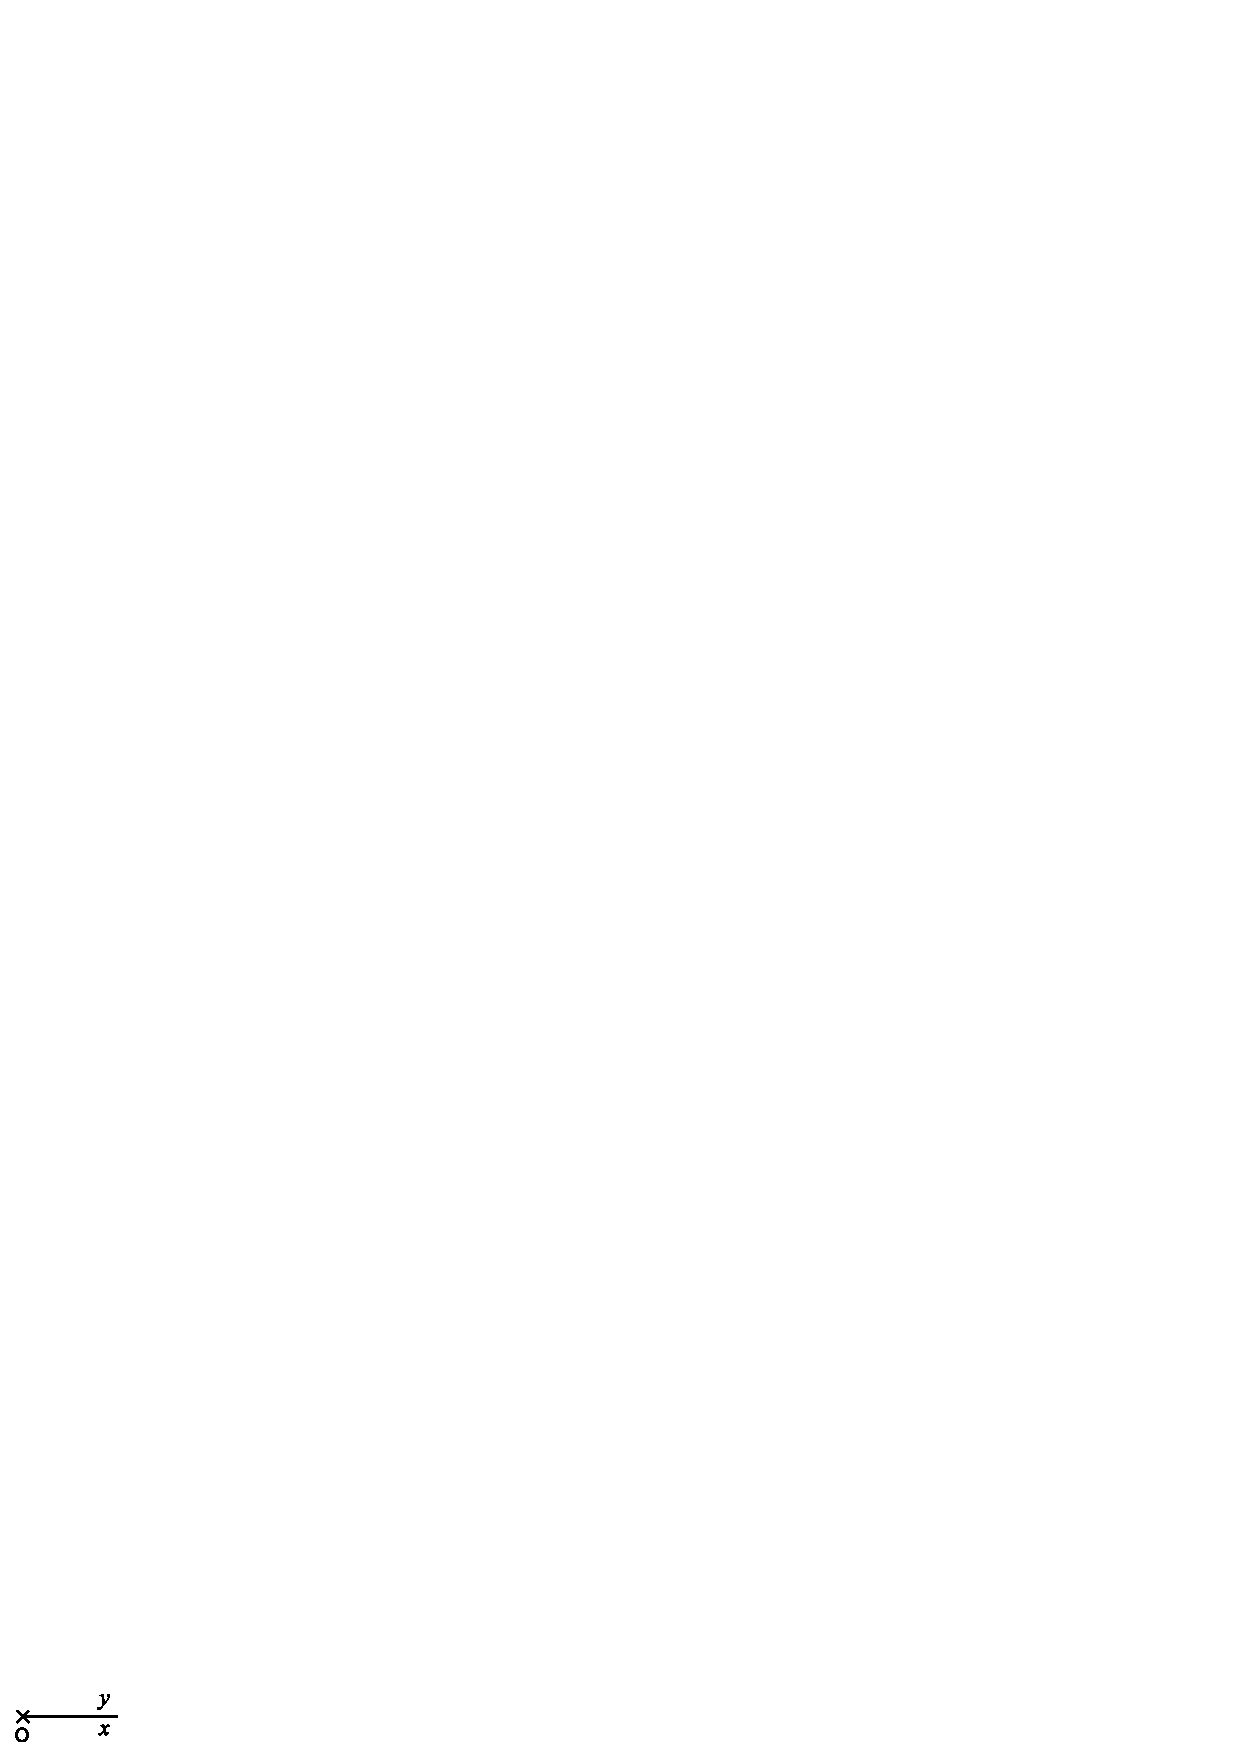
\includegraphics[width=1.7cm]{angle_nul}	&	
\includegraphics[width=1.7cm]{angle_aigu}	&	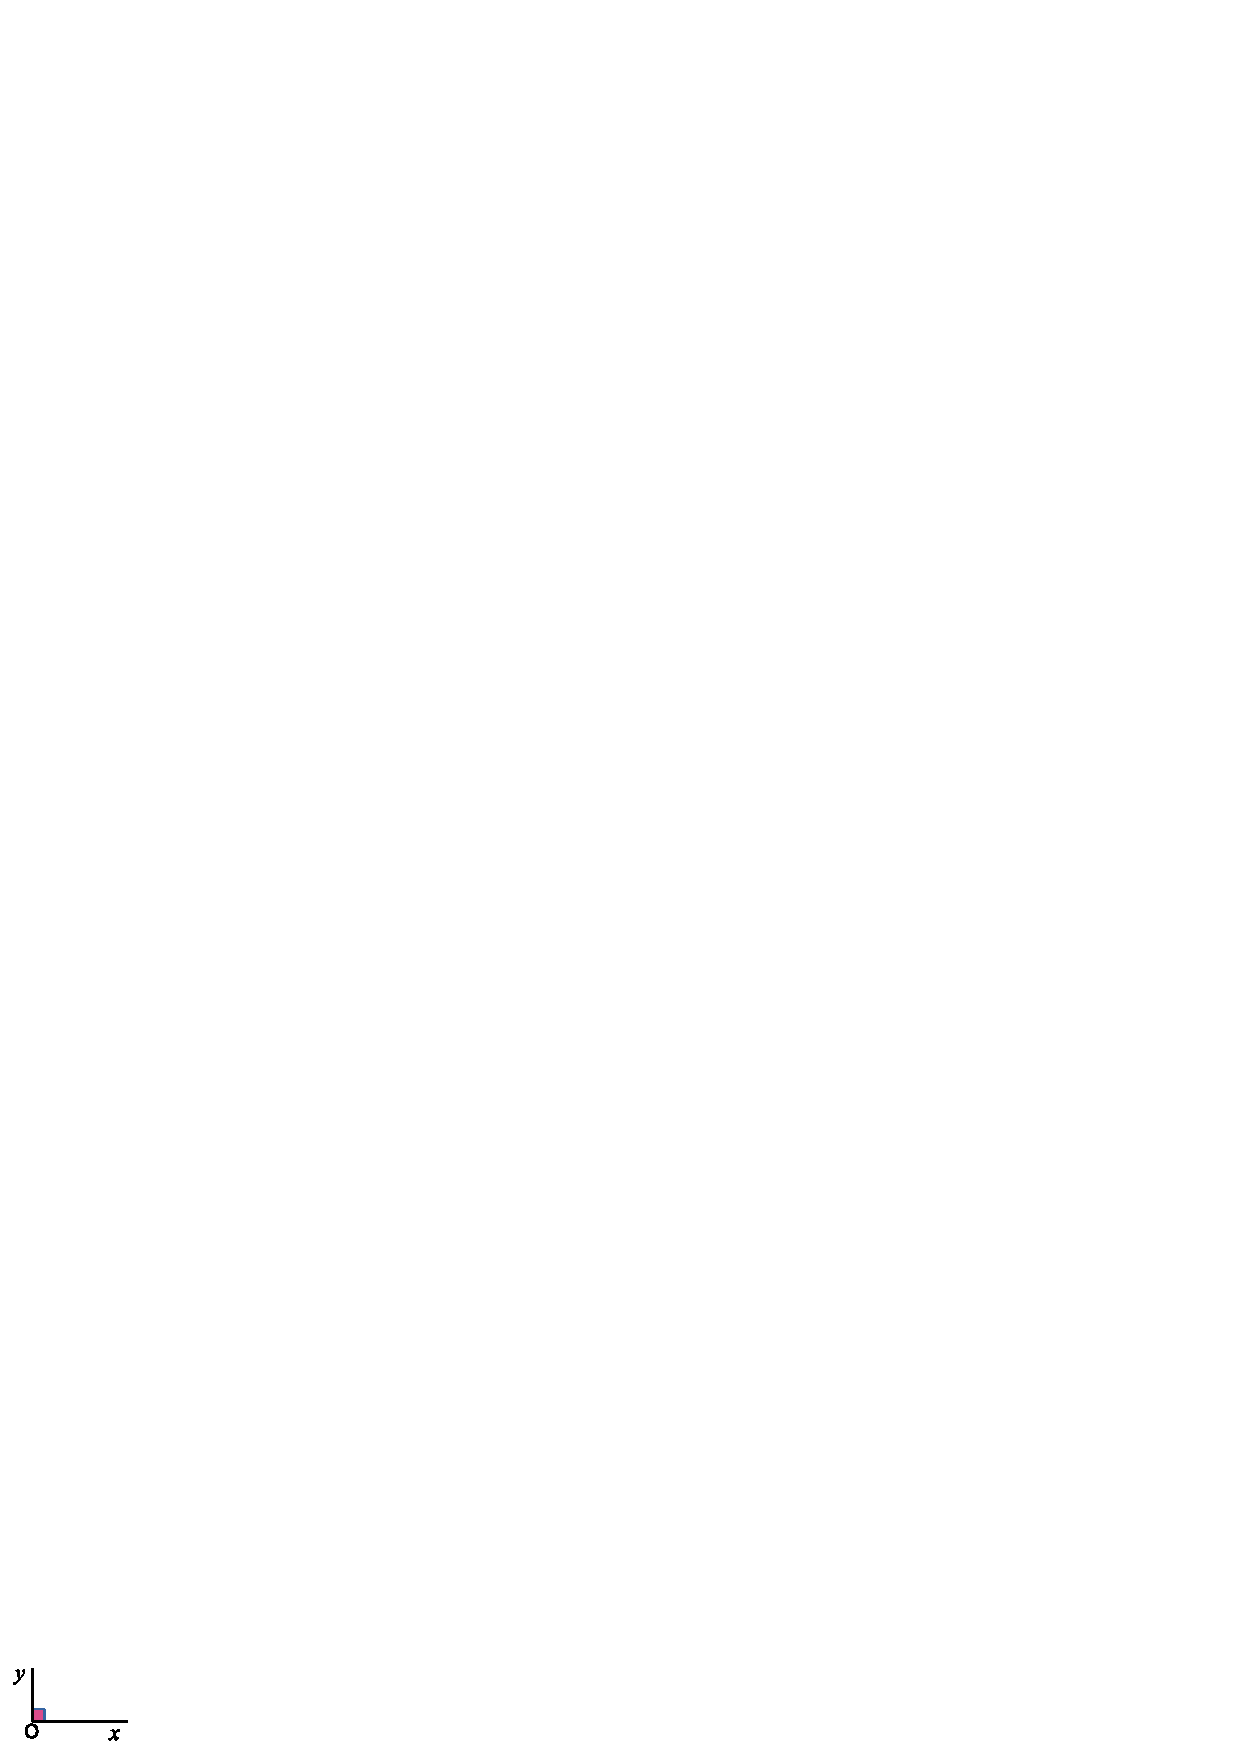
\includegraphics[width=1.7cm]{angle_droit}	&	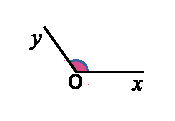
\includegraphics[width=1.7cm]{angle_obtus}	&	
\includegraphics[width=1.7cm]{angle_plat}	\\ \hline
 \textbf{Mesure} 	&	$0^\circ$	&	entre $0^\circ$ et $90^\circ$	&	$90^\circ$		&	entre $90^\circ$ et $180^\circ$	&	 $180^\circ$	\\ \hline
 \multirow{3}{*}{} \textbf{Position} 	&		&	&	&	&	dans le 	\\ 
 \textbf{des}	&	confondus		&	&	perpendiculaires	&	&	 prolongement	\\
\textbf{côtés}	&	&	&	&	&	 l'un de l'autre	\\ \hline
 \end{ttableau}

%%%%%%%%%%%%%%%%%%%%%%%%%%%%%

\begin{methode*1}[Nommer un angle]

\begin{exemple*1}
Nomme l'angle marqué en violet sur la figure ci‑dessous.  \\[0.75em]

\begin{minipage}[c]{0.70\textwidth}
Le sommet de l'angle est le point $C$ : c'est la lettre centrale. \\[0.5em]
Les côtés de l'angle sont les demi‑droites $[CH)$ (ou $[Cx)$) et $[CS)$ (ou $[CA)$ (ou $[Cy)$). \\[0.5em]
Cet angle peut se nommer : $\widehat{{\textcolor{A1}{H}}C{\textcolor{C1}{S}}}$; $\widehat{{\textcolor{C1}{S}}C{\textcolor{A1}{H}}}$ ; $\widehat{{\textcolor{A1}{H}}C{\textcolor{C1}{A}}}$ ; $\widehat{{\textcolor{C1}{A}}C{\textcolor{A1}{H}}}$ ; $\widehat{{\textcolor{C1}{y}}C{\textcolor{A1}{x}}}$.
 \end{minipage} \hfill%
 \begin{minipage}[c]{0.26\textwidth}
 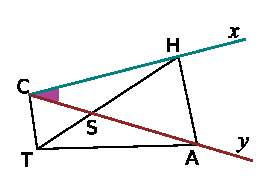
\includegraphics[width=3.8cm]{nommer_angle}
 \end{minipage} \\
 
\end{exemple*1}

\exercice 
Nomme les angles marqués sur la figure ci‑dessous. 
\begin{center} 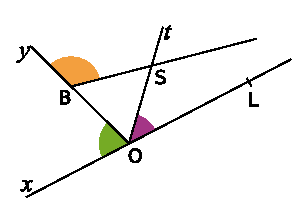
\includegraphics[width=4.5cm]{nommer_angles} \end{center}
%\correction
 
\end{methode*1}

%%%%%%%%%%%%%%%%%%%%%%%%%%%%%

\begin{methode*1}[Utiliser le rapporteur]

\begin{exemple*1}
Mesure l'angle $\widehat{CAB}$. \\[0.75em]

\begin{minipage}[c]{0.49\textwidth}
\centering
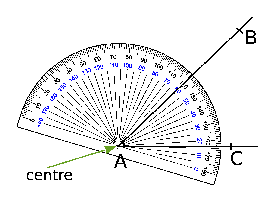
\includegraphics[width=4.8cm]{rapporteur1}
\end{minipage}\hfill%
 \begin{minipage}[c]{0.49\textwidth}%
 \centering
 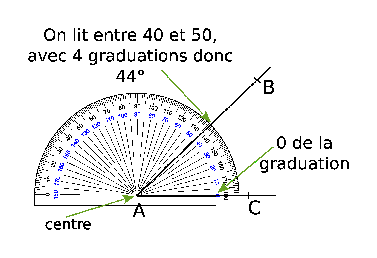
\includegraphics[width=6.6cm]{rapporteur2}
  \end{minipage} \\
 \begin{minipage}[c]{0.43\textwidth}
On place le centre du rapporteur sur le sommet de l'angle.
\end{minipage} \hfill%
 \begin{minipage}[c]{0.53\textwidth}
 On place un zéro du rapporteur sur le côté $[AC)$. Si besoin, on prolonge la demi‑droite $[AC)$. La mesure de l'angle est donnée par l'autre côté de l'angle sur \underline{la même échelle} de graduation.
 \end{minipage} \\
  \end{exemple*1}
 
 \begin{exemple*1}
Construis un angle $\widehat{BUT}$ de $108^\circ$.  \\[0.75em]

\begin{minipage}[c]{0.49\textwidth}
\centering
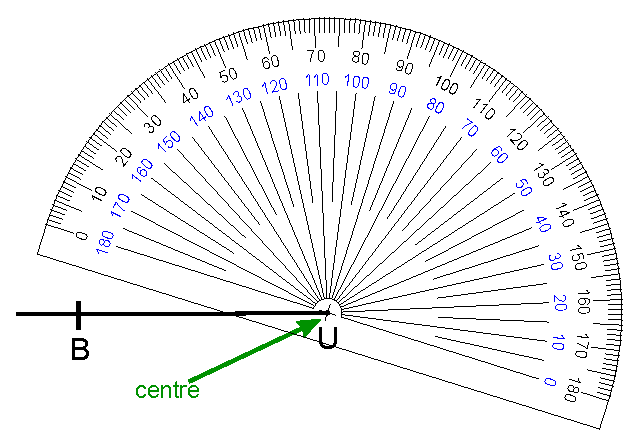
\includegraphics[width=4.8cm]{rapporteur3}
\end{minipage}\hfill%
 \begin{minipage}[c]{0.49\textwidth}%
 \centering
 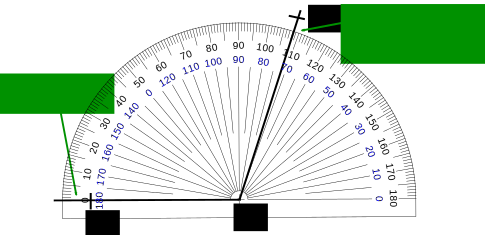
\includegraphics[width=6.6cm]{rapporteur44}
  \end{minipage} \\
 \begin{minipage}[c]{0.43\textwidth}
On trace $[UB)$, premier côté de l'angle. On place le centre du rapporteur sur le point $U$.
\end{minipage} \hfill%
 \begin{minipage}[c]{0.53\textwidth}
 On place un zéro du rapporteur sur le côté $[UB)$. On marque, d'un petit trait-repère, $108^\circ$ avec la bonne graduation.
On trace la demi‑droite d'origine $U$ passant par le repère. On place un point $T$ sur cette demi‑droite.
  \end{minipage} \\
  \end{exemple*1}
 
\exercice
 \begin{enumerate}
 \begin{minipage}[c]{0.36\textwidth}
  \item Mesure l'angle $\widehat{xOy}$ ci‑contre ;
  \item Construis un angle $\widehat{SAT}$ de $85^\circ$. 
  \end{minipage} \hfill%
 \begin{minipage}[c]{0.56\textwidth}
  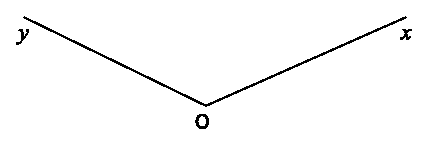
\includegraphics[width=6cm]{angleyOx} 
  \end{minipage} \\
  \end{enumerate}
%\correction
 
\end{methode*1}

%%%%%%%%%%%%%%%%%%%%%%%%%%%%%


\section{La bissectrice}

\begin{definition}
La \textbf{\MotDefinition{bissectrice}{}} d'un angle est la demi-droite qui a pour origine le sommet de l'angle et qui partage l'angle en deux angles de même mesure.
\end{definition}


\begin{methode*1}[Construire une bissectrice]


\begin{exemple*1} \\[0.75em]
Trace un angle $\widehat{xOy}$. Construis sa bissectrice au compas. \\[0.5em]

\begin{tabularx}{\textwidth}{X|X|X}
 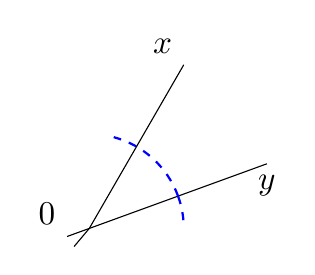
\begin{tikzpicture}[scale=0.6,rotate=20,every node/.style={scale=1.2}]

\draw (-0.5,0) node[above left]{0}--(4,0) node[below]{$y$};
\draw (0,0) --(40:4) node[above left]{$x$};
\draw (0,0)--+(210:0.5);
\draw[thick,dashed,blue] (2,0) arc (0:55:2);
\draw[thick,dashed,blue] (2,0) arc (0:-15:2);

\coordinate (A) at (0,0) ;
\coordinate (B) at (1.414,1.414) ;


\begin{scope}[scale=0.35]
\Compas{A}{B}
\end{scope}


\end{tikzpicture}

 &  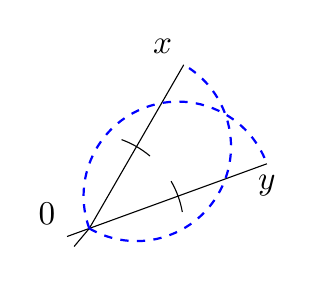
\begin{tikzpicture}[scale=0.6,rotate=20,every node/.style={scale=1.2}]

\draw (-0.5,0) node[above left]{0}--(4,0) node[below]{$y$};
\draw (0,0) --(40:4) node[above left]{$x$};
\draw (0,0)--+(210:0.5);

\draw (1.532,1.286) arc (40:50:2);
\draw (1.532,1.286) arc (40:30:2);
\draw (2,0) arc (0:10:2);
\draw (2,0) arc (0:-10:2);

\draw [thick,blue,dashed](0,0) arc (180:0:2);
\draw [thick,blue,dashed](0,0) arc (-140:40:2);

%\draw (2,0) node{$\bullet$};
%\draw (1.532,1.286) node{$\bullet$};
%\draw (0,0)--(4.698,1.71);

\coordinate (A) at (1.532,1.286) ;
\coordinate (B) at (3.064,2.572) ;

\begin{scope}[scale=0.35]
\Compas{A}{B}
\end{scope}


\end{tikzpicture}

 & 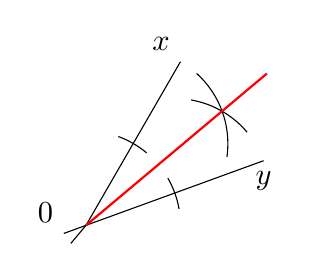
\begin{tikzpicture}[scale=0.6,rotate=20,every node/.style={scale=1.1}]

\draw (-0.5,0) node[above left]{0}--(4,0) node[below]{$y$};
\draw (0,0) --(40:4) node[above left]{$x$};
\draw (0,0)--+(210:0.5);

\draw (1.532,1.286) arc (40:50:2);
\draw (1.532,1.286) arc (40:30:2);
\draw (2,0) arc (0:10:2);
\draw (2,0) arc (0:-10:2);
\draw (3,1.732) arc (60:20:2);
\draw (3.3,2.221) arc (28:-28:2);

\draw [red,thick](0,0)--(4.698,1.71);


\end{tikzpicture}

 \\ 
Au compas, on trace un arc de cercle de centre $O$ qui coupe chaque côté de l'angle en un point. & On trace deux arcs de cercle de même rayon ayant ces deux points pour centres. Ces arcs se coupent en un point. & La bissectrice de l'angle $\widehat{xOy}$ est la demi-droite d'origine $O$ passant par ce point. \\
\end{tabularx} \\

 \end{exemple*1}

\exercice 

Trace un triangle $ABC$ tel que $AB=4$\,cm ; $AC=7$\,cm ; $BC=5$\,cm ; puis trace les bissectrices des angles $\widehat{ABC}$ ; $\widehat{BAC}$ et $\widehat{ACB}$. Que remarques-tu ?

%\correction

 
\end{methode*1}

%%%%%%%%%%%%%%%%%%%%%%%%%%%%%

%%%%%%%%Mise en page
\newpage
%%%%%%%%%%%%%%%%%%%%



\section{Le cercle}

\begin{definition}
Un \textbf{\MotDefinition{cercle}{}} de centre $O$ est l'ensemble des points situés à la même distance du point $O$. 
Cette distance est le \textbf{\MotDefinition{rayon}{}} du cercle.
\end{definition}

\begin{aconnaitre}
\begin{tabularx}{.95\linewidth}{|X|p{5cm}|p{3cm}|}
\hline
\multirow{5}{*}{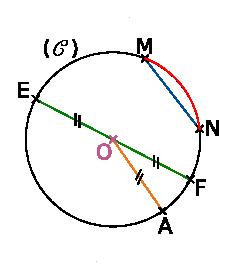
\includegraphics[width=3.4cm]{cercleAFNME}}  & Le \textcolor{C2}{\textbf{centre}} d'un cercle est le point équidistant de tous les points qui constituent ce cercle. & Le point $O$ est le \textcolor{C2}{\textbf{centre}} du cercle $(\mathcal{C})$.\\ \cline{2-3}
 & Un \textcolor{J1}{\textbf{rayon}} d'un cercle est un segment ayant pour extrémités le centre et un point de ce cercle. & Le segment $[OA]$ est un  \textcolor{J1}{\textbf{rayon}} du cercle $(\mathcal{C})$.\\ \cline{2-3}
  & Un  \textcolor{H1}{\textbf{diamètre}} d'un cercle est un segment ayant pour extrémités deux points de ce cercle et contenant son centre. & Le segment $[EF]$ est un  \textcolor{H1}{\textbf{diamètre}} du cercle $(\mathcal{C})$.\\ \cline{2-3}
 & Une  \textcolor{PartieFonction}{\textbf{corde}} d'un cercle est un segment ayant pour extrémités deux points de ce cercle. & Le segment $[MN]$ est une  \textcolor{PartieFonction}{\textbf{corde}} du cercle $(\mathcal{C})$.\\ \cline{2-3}
 & Un  \textcolor{B2}{\textbf{arc de cercle}} est une portion de cercle comprise entre deux points de ce cercle. & La portion de cercle $\overset{\huge{\frown}}{MN}$ comprise entre $M$ et $N$ est un  \textcolor{B2}{\textbf{arc du cercle}} $(\mathcal{C})$.\\ \hline
  \end{tabularx}
 \end{aconnaitre}
  
  
 \begin{remarque}
 Par commodité de langage, on appelle « rayon » la longueur du rayon d'un cercle, et  on appelle « diamètre » la longueur de son diamètre.
  \end{remarque}
  
 \begin{remarque}
 Le diamètre d'un cercle est égal au double de son rayon.
  \end{remarque}

\exercicesbase
\begin{colonne*exercice}

\serie{Points, segments et droites}

\begin{exercice}[Avec un quadrillage]
 \begin{center} 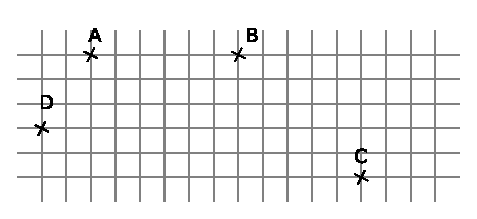
\includegraphics[width=7.2cm]{quadrillage} \end{center}
 \begin{enumerate}
  \item En utilisant le quadrillage de ton cahier, place les points $A$, $B$, $C$ et $D$ comme sur la figure ci-dessus :
  \item Trace en bleu le segment $[AB]$ ;
  \item Trace en vert le segment d'extrémités $D$ et $C$ ;
  \item Trace en rouge la droite passant par $A$ et $C$ ;
  \item Trace en noir la demi-droite d'origine $D$ passant par $B$.
  \end{enumerate}
 \end{exercice}


\begin{exercice}[Appartient ou pas ?]
 \begin{center} 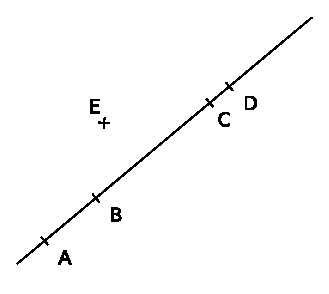
\includegraphics[width=4.8cm]{droiteABECD} \end{center}
 Après avoir observé la figure, recopie et complète les pointillés avec $\in$ ou $\notin$ :
    \begin{colenumerate}{3}
     \item $B$ \ldots $[AC]$ ;
     \item $D$ \ldots $[AB]$ ;
     \item $E$ \ldots $[AD]$ ;
     \item $B$ \ldots $[CA)$ ;
     \item $D$ \ldots $[CA)$ ;
     \item $E$ \ldots $[CE]$.
     \end{colenumerate}
\end{exercice}


\begin{exercice}[À trouver]
 \begin{center} 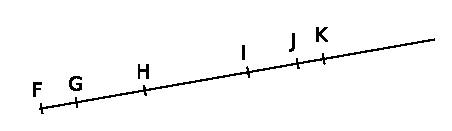
\includegraphics[width=6.5cm]{droiteFGHIJK}  \end{center}
 Parmi les points nommés sur la figure, indique ceux qui appartiennent à :
    \begin{colenumerate}{2}
     \item $[FK]$ ;
     \item $[IG)$ ;
     \item $[FJ]$ et à $[GK]$ ;
     \item $[GJ)$ mais pas à $[HJ]$ ;
     \item $[FG]$ ou à $[IJ)$ ;
     \item $[FH]$ et à $[JK]$.
     \end{colenumerate}
\end{exercice}


\begin{exercice}[Vrai ou faux ?]
 \begin{center} 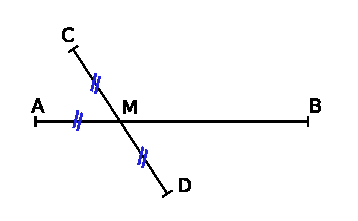
\includegraphics[width=4.6cm]{segmentsAB-CD}  \end{center}
 Observe cette figure composée de deux segments $[AB]$ et $[CD]$ sécants et indique pour chaque affirmation si elle est vraie ou fausse :
 \begin{enumerate}
  \item Les points $C$, $D$ et $M$ sont alignés ;
  \item $M$ est le point d'intersection de $[AB]$ et $[CD]$ ;
  \item $M$ est le milieu du segment $[AC]$ ;
  \item $M$ est un point du segment $[CD]$ ;
  \item $A$ appartient au segment $[MB]$ ;
  \item $M$ est le milieu du segment $[CD]$.
 \end{enumerate}
\end{exercice}


\begin{exercice}[Milieux]
\begin{enumerate} 
 \item Trace un segment $[RS]$ de longueur 4,8 cm et place son milieu $T$ ;
 \item Place un point $U$ qui ne soit pas aligné avec $R$ et $S$ ;
 \item Place le point $V$ tel que $T$ soit le milieu de $[UV]$.
 \end{enumerate}
\end{exercice}


\begin{exercice}[À construire]
\begin{enumerate} 
 \item Place trois points $A$, $B$ et $C$ non alignés ;
 \item Trace les segments $[BC]$ et $[AC]$ ;
 \item Marque le milieu $I$ du segment $[BC]$ et le milieu $J$ du segment $[AC]$ ;
 \item Trace le segment d'extrémités $B$ et $J$ ;
 \item Note $K$ le point d'intersection de $[AI]$ et $[BJ]$ ;
 \item Trace le segment $[AB]$ et place son milieu $L$. Trace enfin le segment $[CL]$. Que remarques‑tu ?
 \end{enumerate}
\end{exercice}


\begin{exercice}[À construire (bis)]
\begin{enumerate} 
 \item Place trois points $L$, $M$ et $N$ non alignés ;
 \item Place un point $A$ appartenant au segment $[LN]$ ;
 \item Place un point $B$ appartenant à la demi‑droite $[MN)$ mais n'appartenant pas au segment $[MN]$ ;
 \item Place le point $C$ aligné d'une part avec $A$ et $B$, et d'autre part avec $L$ et $M$.
 \end{enumerate}
\end{exercice}



%%%%%%%%%%%%%%%%%%%%Mise en page
\vspace{1em}
%%%%%%%%%%%%%%%%%%%%%%%%%%%%%%%



\begin{exercice}[Bande dessinée]
 \begin{center} 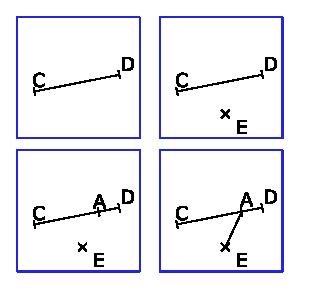
\includegraphics[width=4.3cm]{bande-dessinee}  \end{center}
Pour chaque étape de la bande dessinée, écris la consigne qui a été donnée, sans tenir compte des mesures.
\end{exercice}

%%%%%%%%%%%%%%%%%%%%%%%%%%%%%%%%%%%%%%%%%%%%%%%%%%%%%%%%%

\serie{Droites parallèles et perpendiculaires}

\begin{exercice}[Position de droites]
 \begin{center} 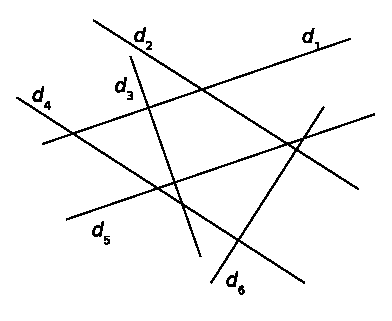
\includegraphics[width=5.8cm]{mikado}  \end{center}
Observe la figure ci‑dessus et note sur ton cahier :
\begin{itemize}
 \item Le nom des droites qui \textbf{te semblent} perpendiculaires ;
 \item Le nom des droites qui sont sécantes mais non perpendiculaires ;
 \item Le nom des droites qui \textbf{te semblent} parallèles.
 \end{itemize}
\end{exercice}


\begin{exercice}[Position de droites (bis)]
 \begin{center} 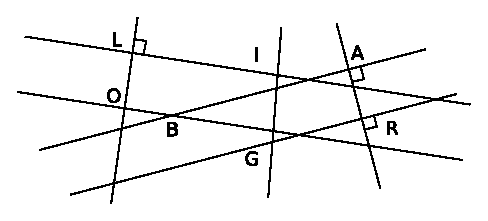
\includegraphics[width=7.3cm]{mikado2}  \end{center}
\begin{enumerate}
 \item Quelles sont les droites qui sont à coup sûr perpendiculaires ?
 \item Quelle semble être la position relative des droites $(BA)$ et $(GR)$ ?
 \end{enumerate}
\end{exercice}


\begin{exercice}[Quadrillage]
Reproduis une figure similaire à celle ci‑dessous. Trace, à la règle, la droite $d_1$ perpendiculaire à la droite $d$ passant par le point $M$ et la droite $d_2$ parallèle à la droite $d'$ passant par $M$.
\begin{center} 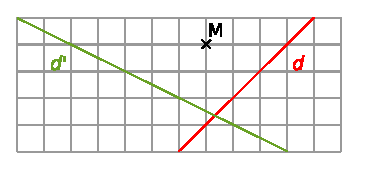
\includegraphics[width=5.2cm]{quadrillage2}  \end{center}
\end{exercice}


\begin{exercice}[Constructions]
\begin{enumerate}
 \item Reproduis sur une feuille blanche les deux figures ci‑dessous :
 \begin{center} 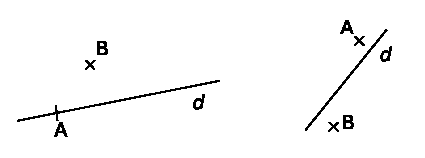
\includegraphics[width=6.1cm]{constructions}  \end{center}
 \item Pour chacune des figures, trace :
  \begin{itemize}
   \item La droite $d'$ perpendiculaire à $d$ et passant par $B$ ;
   \item La droite $d''$ perpendiculaire à $d$ et passant par $A$.
   \end{itemize}
 \item Que peux‑tu dire des droites $d'$ et $d''$ ?
 \end{enumerate}
\end{exercice}


\begin{exercice}[Constructions (bis)]
 \begin{center} \includegraphics[width=5.7cm]{constructions2}  \end{center}
\begin{enumerate}
 \item Reproduis la figure ci‑dessus ;
 \item Trace $d'$, la parallèle à $d$ passant par $A$ ;
 \item Trace $d''$, la parallèle à $d$ passant par $B$ ;
 \item Que peux‑tu dire des droites $d'$ et $d''$ ?
 \end{enumerate}
\end{exercice}


%%%%%%%%%%%%%%%%%%%%Mise en page
\newpage
%%%%%%%%%%%%%%%%%%%%%%%%%%%%%%%



\begin{exercice}[Programme de construction]
\begin{enumerate}
 \item Place deux points $A$ et $B$ tels que $AB = 8$ cm ;
 \item Place un point $L$ sur $[AB]$ tel que $AL = 3$ cm ;
 \item Trace la droite $d$ telle que $L \in d$ et $(AB) \perp d$ ;
 \item Place un point $C$ tel que $C \in d$ et $LC = 2$ cm ;
 \item Trace la droite $d'$ telle que $d' \parallel (AB)$ et $C \in d'$ ;
 \item Sur la demi‑droite $[BC)$, place le point $I$ tel que $BI = 7$ cm ;
 \item Trace la droite $d''$ telle que $I \in d''$ et $d'' \parallel (AC)$.
 \end{enumerate}
\end{exercice}


\begin{exercice}
Construis la figure suivante : \\[0.75em]
\begin{minipage}[c]{0.2\textwidth}
\includegraphics[width=3.8cm]{constructions3}
 \end{minipage} \hfill%
 \begin{minipage}[c]{0.2\textwidth}
 $(BM) \parallel (AN)$
  \end{minipage} \\
\end{exercice}


\begin{exercice}
Reproduis la figure ci‑dessous en vraie grandeur : \\[0.75em]
\begin{minipage}[c]{0.3\textwidth}
\includegraphics[width=4.5cm]{double-triangle}
 \end{minipage} \hfill%
 \begin{minipage}[c]{0.4\textwidth}
$AB = 5,3$ cm ;

$BC = 3$ cm ;

$AC = 7,7$ cm.
 \end{minipage} \\
\end{exercice}

%%%%%%%%%%%%%%%%%%%%%%%%%%%%%%%%%%%%%%%%%%%%%%%%%%%%%%%%%

\serie{Médiatrice d’un segment}

\begin{exercice}[Médiatrices]
Dans chaque cas, trace le segment de longueur donnée puis sa médiatrice :
 \begin{colenumerate}{3}
  \item $AB = 2$ cm ;
  \item $DE = 7,8$ cm ;
  \item $FG = 76$ mm.
  \end{colenumerate}
\end{exercice}


\begin{exercice}[Points alignés]
 \begin{enumerate}
  \item Trace un segment $[AB]$ de longueur 7 cm ;
  \item Place le point $C$ de la demi‑droite $[BA)$ tel que $BC = 12$ cm ;
  \item Construis la médiatrice $m_1$ du segment $[AC]$ ;
  \item Construis la médiatrice $m_2$ du segment $[AB]$ ;
  \item Que remarques‑tu ?
  \end{enumerate}
\end{exercice}


\begin{exercice}[Reconnaître]
Sur chacune des figures ci‑dessous, indique si $P$ est sur la médiatrice de $[AB]$ : \\[0.5em]
 \begin{colenumerate}{2}
  \item 
  
  \includegraphics[width=2.2cm]{mediatriceAB1}
  \item 
  
  \includegraphics[width=2.2cm]{mediatriceAB2}
  \item 
  
  \includegraphics[width=2.2cm]{mediatriceAB3}
  \item 
  
  \includegraphics[width=2.2cm]{mediatriceAB4}
  \end{colenumerate}
\end{exercice}
 
 
\begin{exercice}[Construction]
 \begin{enumerate}
 \item Trace un segment $[AB]$ de longueur 6 cm ;
 \item Construis la médiatrice $d$ du segment $[AB]$ au compas ;
 \item Place un point $M$ sur $d$ à 7 cm de $A$ ;
 \item Quelle est la longueur de $[BM]$ ? 
 
Tu la justifieras en utilisant une propriété.
  \end{enumerate}
\end{exercice}


\begin{exercice}[Concours de médiatrices]
 \begin{enumerate}
 \item Place trois points $A$, $B$ et $C$ non alignés ;
 \item Trace sans équerre les médiatrices des segments $[AB]$, $[AC]$ et $[BC]$. 
 
 Que constates‑tu ?
 \end{enumerate}
\end{exercice}


%%%%%%%%%%%%%%%%%%%%Mise en page
\newpage
%%%%%%%%%%%%%%%%%%%%%%%%%%%%%%%



%%%%%%%%%%%%%%%%%%%%%%%%%%%%%%%%%%%%%%%%%%%%%%%%%%%%%%%%%

\serie{Nommer un angle}


\begin{exercice}[De toutes les couleurs]
Les points $A$, $O$ et $L$ sont alignés.
 \begin{center} \includegraphics[width=6.7cm]{angles-colores}  \end{center}
\begin{enumerate}
 \item Nomme les angles marqués en couleur dans la figure de toutes les façons possibles ; 
 \item Reproduis la figure puis marque en bleu l'angle $\widehat{yOz}$, en rouge l'angle $\widehat{PMC}$ et en vert l'angle $\widehat{PAL}$.
 \end{enumerate}
\end{exercice}


\begin{exercice}[Plusieurs noms]
Les segments $[TD]$ et $[PS]$ sont sécants en $A$ et les segments $[PI]$ et $[TD]$ se coupent en $R$.

Trouve toutes les autres façons de nommer : \\[0.5em]
\begin{minipage}[c]{0.2\textwidth}
\begin{itemize}
 \item l'angle $\widehat{APR}$ ;
 \item l'angle $\widehat{RDI}$ ;
 \item l'angle $\widehat{PDA}$.
 \end{itemize}
 \end{minipage} \hfill%
  \begin{minipage}[c]{0.4\textwidth}
  \includegraphics[width=4.7cm]{segments-secants}
  \end{minipage} \\
\end{exercice}  


\begin{exercice}[Quelle étourdie !]
Louise a recopié la figure ci‑dessous qui était au tableau mais elle a oublié de noter les noms des points d'intersection des droites. 
 \begin{center} \includegraphics[width=5.2cm]{angles-multicolores}  \end{center}
Elle appelle son camarade Ahmed qui lui dit que les angles en couleur se nomment $\widehat{ABC}$, $\widehat{DBA}$, $\widehat{FAC}$ et $\widehat{FAE}$. \\[0.5em]
Reproduis la figure et nomme les points grâce à ces indications.
\end{exercice}  


%%%%%%%%%%%%%%%%%%%%Mise en page
\vspace{3em}
%%%%%%%%%%%%%%%%%%%%%%%%%%%%%%%




%%%%%%%%%%%%%%%%%%%%%%%%%%%%%%%%%%%%%%%%%%%%%%%%%%%%%%%%%

\serie{Mesure d'un angle}


\begin{exercice}[À vue d’œil]
\prof
{ce travail sera fait de façon approxiamtive; il peut être sujet à discussion.}

Indique les angles qui te paraissent obtus, aigus ou droits.
 \begin{center} \includegraphics[width=7cm]{angles-toutgenre}  \end{center}
\end{exercice}


\begin{exercice}[Avec l'équerre]
\prof
{Ce travail sera fait de façon approxiamtive; il peut être sujet à discussion.}

En utilisant ton équerre, détermine quels sont les angles aigus, obtus ou droits dans chacun des cas ci-dessous.
 \begin{center} \includegraphics[width=7cm]{angles-droits}  \end{center}
\end{exercice}

%%%%%%%%%%%%%%%%%%%%Mise en page
\newpage
%%%%%%%%%%%%%%%%%%%%%%%%%%%%%%%

\begin{exercice}[Bien placé ?]
%Dans chacun des cas suivants, José souhaite mesurer l'angle $\widehat{BAC}$.

%Peut‑il effectuer une mesure correcte ? Si oui, indique la mesure de l'angle et si non, explique pourquoi. \\[0.5em]
\begin{colenumerate}{2}
%%%%%%%%%%%%%%%%%%%%%%%%%%%%%%%%%%%%%%%%%%%%%%%%%%%
%Rapporteur 1
%%%%%%%%%%%%%%%%%%%%%%%%%%%%%%%%%%%%%%%%%%%%%%%%%%%
 \item  %\includegraphics[width=3.6cm]{rapporteurA}

\scalebox{.8}{
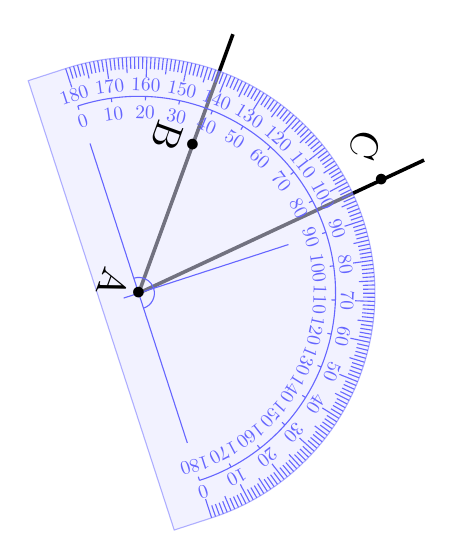
\begin{tikzpicture}

\def \RotFigure {-110} %rotation de toute la figure y compris textes
\begin{scope}[rotate=\RotFigure]

\def \CharSize {1.4};
\def \BulletSize {1};
\coordinate (A) at (0,0);
\coordinate (B) at (-2,0);
\coordinate (C) at (-2.404,2.404);
\coordinate (U) at (-3.5,0);
\coordinate (V) at (-2.828,2.828);

\draw[line width = 1.3pt] (U) -- (A) -- (V);
	
%début du rapporteur
    %Définition de l 'angle de rotation du rapporteur
    \def \RapRot {38} 
    %Définition du décalage du rapporteur
    \def \DecalX {0}
    \def \DecalY {0}
    %Couleur des élèments du rapporteur (sauf le remplissage)
    \def \RapColor {blue!60}
\begin{scope}[shift={(\DecalX,\DecalY)},rotate=\RapRot]
    % contours du rapporteur
    \draw[color=\RapColor, fill =blue!10, opacity=0.5] (-3,0) arc(180:0:3)--(3,-0.5)--(-3,-0.5)--cycle;	%Dont couleur de remplissage
    \draw[color=\RapColor] (-2,0)--(2,0);
    \draw[color=\RapColor] (0,-0.2)--(0,2);
    % graduation externe 1 degrés
    \foreach \a in {0,1,...,180}{\draw[color=\RapColor] (\a:3)--(\a:2.85);}
    % graduation externe 5 degrés
    \foreach \a in {0,5,...,180}{\draw[color=\RapColor] (\a:2.85)--(\a:2.8);}
    % double graduation
   \foreach \a/\b in {%
        0/-90,10/-80,20/-70,30/-60,40/-50,50/-40,%
        60/-30,70/-20,80/-10,90/0,100/10,110/20,%
        120/30,130/40,140/50,150/60,160/70,170/80,180/90%
    }{
    % graduation externe 10 degrés
    \draw[color=\RapColor] (\a:2.80)--(\a:2.75) 
    node[scale=0.7, rotate=\b+\RapRot+\RotFigure] (\a) at (\a:2.65){\a};
    % graduation interne 10 degrés
    \draw[color=\RapColor] (\a:2.5)--(\a:2.45)
	node[thin,scale=0.7, rotate=-\b+\RapRot+\RotFigure] (\a) at (180-\a:2.3){\a}; }
    % demi-cercle intérieur
    \draw[color=\RapColor](-2.5,0) arc(180:0:2.5);
    %demi-cercle à l'origine
    \draw[color=\RapColor](-0.2,0) arc(180:0:0.2);
\end{scope}
%fin du rapporteur

\draw (A) node [below,scale=\CharSize,rotate=\RotFigure]{A};
\draw (A) node[scale=\BulletSize]{$\bullet$};
\draw (B) node [below,scale=\CharSize,rotate=\RotFigure]{B};
\draw (B) node[scale=\BulletSize]{$\bullet$};
\draw (C) node [below left,scale=\CharSize,rotate=\RotFigure]{C};
\draw (C) node[scale=\BulletSize]{$\bullet$};
\end{scope}
\end{tikzpicture}
}


\item  %\vspace{-2em} \includegraphics[width=3.6cm]{rapporteurB}
%%%%%%%%%%%%%%%%%%%%%%%%%%%%%%%%%%%%%%%%%%%%%%%%%%%
%Rapporteur 2
%%%%%%%%%%%%%%%%%%%%%%%%%%%%%%%%%%%%%%%%%%%%%%%%%%%

\scalebox{.8}{
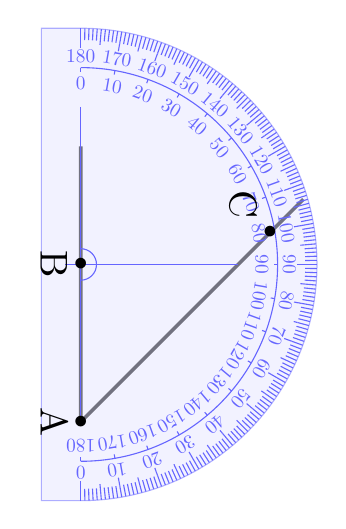
\begin{tikzpicture}

\def \RotFigure {-90} %rotation de toute la figure y compris textes
\begin{scope}[rotate=\RotFigure]

\def \CharSize {1.4};
\def \BulletSize {1};
\coordinate (A) at (0,0);
\coordinate (B) at (-2,0);
\coordinate (C) at (-2.404,2.404);
\coordinate (U) at (-3.5,0);
\coordinate (V) at (-2.828,2.828);

\draw[line width = 1.3pt] (U) -- (A) -- (V);
	
%début du rapporteur

    %Définition de l 'angle de rotation du rapporteur
    \def \RapRot {0} 
    %Définition du décalage du rapporteur
    \def \DecalX {-2}
    \def \DecalY {0}
    %Couleur des élèments du rapporteur (sauf le remplissage)
    \def \RapColor {blue!60}

\begin{scope}[shift={(\DecalX,\DecalY)},rotate=\RapRot]
    % contours du rapporteur
    \draw[color=\RapColor, fill =blue!10, opacity=0.5] (-3,0) arc(180:0:3)--(3,-0.5)--(-3,-0.5)--cycle;	%Dont couleur de remplissage
    \draw[color=\RapColor] (-2,0)--(2,0);
    \draw[color=\RapColor] (0,-0.2)--(0,2);
    % graduation externe 1 degrés
    \foreach \a in {0,1,...,180}{\draw[color=\RapColor] (\a:3)--(\a:2.85);}
    % graduation externe 5 degrés
    \foreach \a in {0,5,...,180}{\draw[color=\RapColor] (\a:2.85)--(\a:2.8);}
    % double graduation
   \foreach \a/\b in {%
        0/-90,10/-80,20/-70,30/-60,40/-50,50/-40,%
        60/-30,70/-20,80/-10,90/0,100/10,110/20,%
        120/30,130/40,140/50,150/60,160/70,170/80,180/90%
    }{
    % graduation externe 10 degrés
    \draw[color=\RapColor] (\a:2.80)--(\a:2.75) 
    node[scale=0.7, rotate=\b+\RapRot+\RotFigure] (\a) at (\a:2.65){\a};
    % graduation interne 10 degrés
    \draw[color=\RapColor] (\a:2.5)--(\a:2.45)
	node[thin,scale=0.7, rotate=-\b+\RapRot+\RotFigure] (\a) at (180-\a:2.3){\a}; }
    % demi-cercle intérieur
    \draw[color=\RapColor](-2.5,0) arc(180:0:2.5);
    %demi-cercle à l'origine
    \draw[color=\RapColor](-0.2,0) arc(180:0:0.2);
\end{scope}
%fin du rapporteur

\draw (A) node [below,scale=\CharSize,rotate=\RotFigure]{A};
\draw (A) node[scale=\BulletSize]{$\bullet$};
\draw (B) node [below,scale=\CharSize,rotate=\RotFigure]{B};
\draw (B) node[scale=\BulletSize]{$\bullet$};
\draw (C) node [below left,scale=\CharSize,rotate=\RotFigure]{C};
\draw (C) node[scale=\BulletSize]{$\bullet$};
\end{scope}
\end{tikzpicture}
}

 \item %\includegraphics[width=3.6cm]{rapporteurC}
%%%%%%%%%%%%%%%%%%%%%%%%%%%%%%%%%%%%%%%%%%%%%%%%%%%
%Rapporteur 3
%%%%%%%%%%%%%%%%%%%%%%%%%%%%%%%%%%%%%%%%%%%%%%%%%%%

\scalebox{.8}{
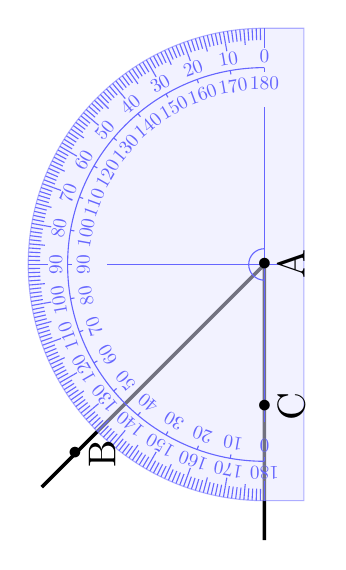
\begin{tikzpicture}

\def \RotFigure {-90} %rotation de toute la figure y compris textes
\begin{scope}[rotate=\RotFigure]

\def \CharSize {1.4};
\def \BulletSize {1};
\coordinate (A) at (0,0);
\coordinate (B) at (2.404,-2.404);
\coordinate (C) at (1.8,0);
\coordinate (U) at (3.5,0);
\coordinate (V) at (2.828,-2.828);

\draw[line width = 1.3pt] (U) -- (A) -- (V);
	
%début du rapporteur
    %Définition de l 'angle de rotation du rapporteur
    \def \RapRot {180} 
    %Définition du décalage du rapporteur
    \def \DecalX {0}
    \def \DecalY {0}
    %Couleur des élèments du rapporteur (sauf le remplissage)
    \def \RapColor {blue!60}

\begin{scope}[shift={(\DecalX,\DecalY)},rotate=\RapRot]
    % contours du rapporteur
    \draw[color=\RapColor, fill =blue!10, opacity=0.5] (-3,0) arc(180:0:3)--(3,-0.5)--(-3,-0.5)--cycle;	%Dont couleur de remplissage
    \draw[color=\RapColor] (-2,0)--(2,0);
    \draw[color=\RapColor] (0,-0.2)--(0,2);
    % graduation externe 1 degrés
    \foreach \a in {0,1,...,180}{\draw[color=\RapColor] (\a:3)--(\a:2.85);}
    % graduation externe 5 degrés
    \foreach \a in {0,5,...,180}{\draw[color=\RapColor] (\a:2.85)--(\a:2.8);}
    % double graduation
   \foreach \a/\b in {%
        0/-90,10/-80,20/-70,30/-60,40/-50,50/-40,%
        60/-30,70/-20,80/-10,90/0,100/10,110/20,%
        120/30,130/40,140/50,150/60,160/70,170/80,180/90%
    }{
    % graduation externe 10 degrés
    \draw[color=\RapColor] (\a:2.80)--(\a:2.75) 
    node[scale=0.7, rotate=\b+\RapRot+\RotFigure] (\a) at (\a:2.65){\a};
    % graduation interne 10 degrés
    \draw[color=\RapColor] (\a:2.5)--(\a:2.45)
	node[thin,scale=0.7, rotate=-\b+\RapRot+\RotFigure] (\a) at (180-\a:2.3){\a}; }
    % demi-cercle intérieur
    \draw[color=\RapColor](-2.5,0) arc(180:0:2.5);
    %demi-cercle à l'origine
    \draw[color=\RapColor](-0.2,0) arc(180:0:0.2);
\end{scope}
%fin du rapporteur

\draw (A) node [below,scale=\CharSize,rotate=-\RotFigure]{A};
\draw (A) node[scale=\BulletSize]{$\bullet$};
\draw (B) node [below,scale=\CharSize,rotate=-\RotFigure]{B};
\draw (B) node[scale=\BulletSize]{$\bullet$};
\draw (C) node [below,scale=\CharSize,rotate=-\RotFigure]{C};
\draw (C) node[scale=\BulletSize]{$\bullet$};
\end{scope}
\end{tikzpicture}
}

 \item  %\includegraphics[width=3.6cm]{rapporteurD}
%%%%%%%%%%%%%%%%%%%%%%%%%%%%%%%%%%%%%%%%%%%%%%%%%%%
%Rapporteur 4
%%%%%%%%%%%%%%%%%%%%%%%%%%%%%%%%%%%%%%%%%%%%%%%%%%%

\scalebox{.8}{
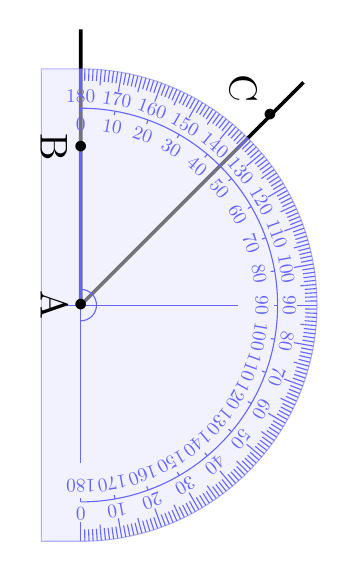
\begin{tikzpicture}

\def \RotFigure {-90} %rotation de toute la figure y compris textes
\begin{scope}[rotate=\RotFigure]

\def \CharSize {1.4};
\def \BulletSize {1};
\coordinate (A) at (0,0);
\coordinate (B) at (-2,0);
\coordinate (C) at (-2.404,2.404);
\coordinate (U) at (-3.5,0);
\coordinate (V) at (-2.828,2.828);

\draw[line width = 1.3pt] (U) -- (A) -- (V);
\draw (-0.5,0);
	
%début du rapporteur
    %Définition de l 'angle de rotation du rapporteur
    \def \RapRot {0} 
    %Définition du décalage du rapporteur
    \def \DecalX {0}
    \def \DecalY {0}
    %Couleur des élèments du rapporteur (sauf le remplissage)
    \def \RapColor {blue!60}

\begin{scope}[shift={(\DecalX,\DecalY)},rotate=\RapRot]
    % contours du rapporteur
    \draw[color=\RapColor, fill =blue!10, opacity=0.5] (-3,0) arc(180:0:3)--(3,-0.5)--(-3,-0.5)--cycle;	%Dont couleur de remplissage
    \draw[color=\RapColor] (-2,0)--(2,0);
    \draw[color=\RapColor] (0,-0.2)--(0,2);
    % graduation externe 1 degrés
    \foreach \a in {0,1,...,180}{\draw[color=\RapColor] (\a:3)--(\a:2.85);}
    % graduation externe 5 degrés
    \foreach \a in {0,5,...,180}{\draw[color=\RapColor] (\a:2.85)--(\a:2.8);}
    % double graduation
   \foreach \a/\b in {%
        0/-90,10/-80,20/-70,30/-60,40/-50,50/-40,%
        60/-30,70/-20,80/-10,90/0,100/10,110/20,%
        120/30,130/40,140/50,150/60,160/70,170/80,180/90%
    }{
    % graduation externe 10 degrés
    \draw[color=\RapColor] (\a:2.80)--(\a:2.75) 
    node[scale=0.7, rotate=\b+\RapRot+\RotFigure] (\a) at (\a:2.65){\a};
    % graduation interne 10 degrés
    \draw[color=\RapColor] (\a:2.5)--(\a:2.45)
	node[thin,scale=0.7, rotate=-\b+\RapRot+\RotFigure] (\a) at (180-\a:2.3){\a}; }
    % demi-cercle intérieur
    \draw[color=\RapColor](-2.5,0) arc(180:0:2.5);
    %demi-cercle à l'origine
    \draw[color=\RapColor](-0.2,0) arc(180:0:0.2);
\end{scope}
%fin du rapporteur

\draw (A) node [below,scale=\CharSize, rotate=\RotFigure]{A};
\draw (A) node[scale=\BulletSize]{$\bullet$};
\draw (B) node [below,scale=\CharSize, rotate=\RotFigure]{B};
\draw (B) node[scale=\BulletSize]{$\bullet$};
\draw (C) node [below left,scale=\CharSize, rotate=\RotFigure]{C};
\draw (C) node[scale=\BulletSize]{$\bullet$};
\end{scope}
\end{tikzpicture}
}
 
 \item % \includegraphics[width=3.6cm]{rapporteurD}
%%%%%%%%%%%%%%%%%%%%%%%%%%%%%%%%%%%%%%%%%%%%%%%%%%%
%Rapporteur 5
%%%%%%%%%%%%%%%%%%%%%%%%%%%%%%%%%%%%%%%%%%%%%%%%%%%



\scalebox{.8}{
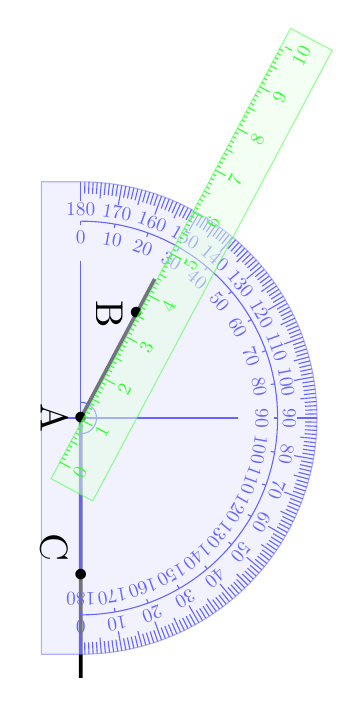
\begin{tikzpicture}

\def \RotFigure {-90} %rotation de toute la figure y compris textes
\begin{scope}[rotate=\RotFigure]

\def \CharSize {1.4};
\def \BulletSize {1};
\coordinate (A) at (0,0);
\coordinate (B) at (-1.324,0.704);
\coordinate (C) at (2,0);
\coordinate (U) at (-1.766,0.939);
\coordinate (V) at (3.3,0);

\draw[line width = 1.3pt] (U) -- (A) -- (V);
	
%début du rapporteur
    %Définition de l 'angle de rotation du rapporteur
    \def \Rotation {0} 
    %Définition du décalage du rapporteur
    \def \DecalX {0}
    \def \DecalY {0}
    %Couleur des élèments du rapporteur (sauf le remplissage)
    \def \RapColor {blue!60}

\begin{scope}[shift={(\DecalX,\DecalY)},rotate=\Rotation]
    % contours du rapporteur
    \draw[color=\RapColor, fill =blue!10, opacity=0.5] (-3,0) arc(180:0:3)--(3,-0.5)--(-3,-0.5)--cycle;	%Dont couleur de remplissage
    \draw[color=\RapColor] (-2,0)--(2,0);
    \draw[color=\RapColor] (0,-0.2)--(0,2);
    % graduation externe 1 degrés
    \foreach \a in {0,1,...,180}{\draw[color=\RapColor] (\a:3)--(\a:2.85);}
    % graduation externe 5 degrés
    \foreach \a in {0,5,...,180}{\draw[color=\RapColor] (\a:2.85)--(\a:2.8);}
    % double graduation
   \foreach \a/\b in {%
        0/-90,10/-80,20/-70,30/-60,40/-50,50/-40,%
        60/-30,70/-20,80/-10,90/0,100/10,110/20,%
        120/30,130/40,140/50,150/60,160/70,170/80,180/90%
    }{
    % graduation externe 10 degrés
    \draw[color=\RapColor] (\a:2.80)--(\a:2.75) 
    node[scale=0.7, rotate=\b+\Rotation+\RotFigure] (\a) at (\a:2.65){\a};
    % graduation interne 10 degrés
    \draw[color=\RapColor] (\a:2.5)--(\a:2.45)
	node[thin,scale=0.7, rotate=-\b+\Rotation+\RotFigure] (\a) at (180-\a:2.3){\a}; }
    % demi-cercle intérieur
    \draw[color=\RapColor](-2.5,0) arc(180:0:2.5);
    %demi-cercle à l'origine
    \draw[color=\RapColor](-0.2,0) arc(180:0:0.2);
\end{scope}
%fin du rapporteur

\draw (A) node [below,scale=\CharSize,rotate=\RotFigure]{A};
\draw (A) node[scale=\BulletSize]{$\bullet$};
\draw (B) node [below,scale=\CharSize,rotate=\RotFigure]{B};
\draw (B) node[scale=\BulletSize]{$\bullet$};
\draw (C) node [below left,scale=\CharSize,rotate=\RotFigure]{C};
\draw (C) node[scale=\BulletSize]{$\bullet$};

	
%début de la règle
    %Graduaton max. de la règle
    \def \TailleRegle {10}
    %Définition de l 'angle de rotation de la règle
    \def \RotationRegle {152}
    %Définition du décalage de la règle
    \def \DecalRegleX {0.7}
    \def \DecalRegleY {0}
    %Couleur des élèments de la règle (sauf le remplissage)
    \def \RegleColor {green!80}

\begin{scope}[shift={(\DecalRegleX,\DecalRegleY)},rotate=\RotationRegle, scale=0.6]
    % contours de la règle
    \draw[color=\RegleColor, fill =green!10, opacity=0.5] (-0.4,0.5) rectangle (\TailleRegle+0.4,-0.5);	%Dont couleur de remplissage
    % graduation 1 mm
    \foreach \a in {0,0.1,...,\TailleRegle}{\draw[color=\RegleColor] (\a,0.5)--(\a,0.42);}
    % graduation 5 mm
    \foreach \a in {0,0.5,...,\TailleRegle}{\draw[color=\RegleColor] (\a,0.42)--(\a,0.35);}
    % graduation et repères 10 mm
    \foreach \a in {0,1,...,\TailleRegle}{\draw[color=\RegleColor] (\a,0.35)--(\a,0.25)
    node[scale=0.7, rotate=\RotationRegle+\RotFigure] (\a) at (\a,0.02){\a};}
    
\end{scope}
%fin de la règle

\end{scope}
\end{tikzpicture}
}

 \item % \vspace{-2em} \includegraphics[width=3.6cm]{rapporteurF}
%%%%%%%%%%%%%%%%%%%%%%%%%%%%%%%%%%%%%%%%%%%%%%%%%%%
%Rapporteur 6
%%%%%%%%%%%%%%%%%%%%%%%%%%%%%%%%%%%%%%%%%%%%%%%%%%%

\scalebox{.8}{
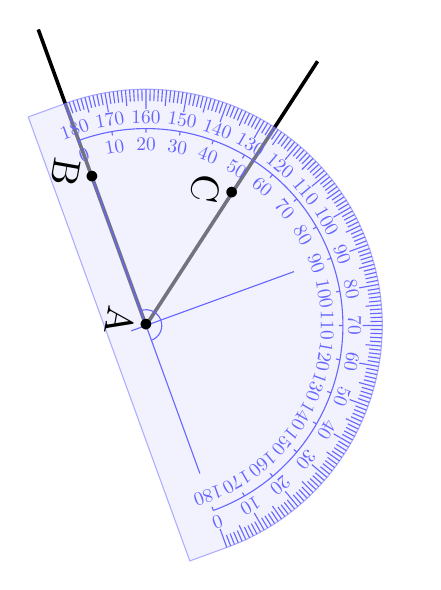
\begin{tikzpicture}

\def \RotFigure {-100} %rotation de toute la figure y compris textes
\begin{scope}[rotate=\RotFigure]

\def \CharSize {1.4};
\def \BulletSize {1};
\coordinate (A) at (0,0);
\coordinate (B) at (-1.732,-1);
\coordinate (C) at (-1.841,0.781);
\coordinate (U) at (-3.464,-2);
\coordinate (V) at (-3.682,1.563);

\draw[line width = 1.3pt] (U) -- (A) -- (V);

%début du rapporteur
    %Définition de l 'angle de rotation du rapporteur
    \def \RapRot {30} 
    %Définition du décalage du rapporteur
    \def \DecalX {0}
    \def \DecalY {0}
    %Couleur des élèments du rapporteur (sauf le remplissage)
    \def \RapColor {blue!60}

\begin{scope}[shift={(\DecalX,\DecalY)},rotate=\RapRot]

    % contours du rapporteur
    \draw[color=\RapColor, fill =blue!10, opacity=0.5] (-3,0) arc(180:0:3)--(3,-0.5)--(-3,-0.5)--cycle;	%Dont couleur de remplissage
    \draw[color=\RapColor] (-2,0)--(2,0);
    \draw[color=\RapColor] (0,-0.2)--(0,2);
    % graduation externe 1 degrés
    \foreach \a in {0,1,...,180}{\draw[color=\RapColor] (\a:3)--(\a:2.85);}
    % graduation externe 5 degrés
    \foreach \a in {0,5,...,180}{\draw[color=\RapColor] (\a:2.85)--(\a:2.8);}
    % double graduation
   \foreach \a/\b in {%
        0/-90,10/-80,20/-70,30/-60,40/-50,50/-40,%
        60/-30,70/-20,80/-10,90/0,100/10,110/20,%
        120/30,130/40,140/50,150/60,160/70,170/80,180/90%
    }{
    % graduation externe 10 degrés
    \draw[color=\RapColor] (\a:2.80)--(\a:2.75) 
    node[scale=0.7, rotate=\b+\RapRot+\RotFigure] (\a) at (\a:2.65){\a};
    % graduation interne 10 degrés
    \draw[color=\RapColor] (\a:2.5)--(\a:2.45)
	node[thin,scale=0.7, rotate=-\b+\RapRot+\RotFigure] (\a) at (180-\a:2.3){\a}; }
    % demi-cercle intérieur
    \draw[color=\RapColor](-2.5,0) arc(180:0:2.5);
    %demi-cercle à l'origine
    \draw[color=\RapColor](-0.2,0) arc(180:0:0.2);
\end{scope}
%fin du rapporteur

\draw (A) node [below,scale=\CharSize,rotate=\RotFigure]{A};
\draw (A) node[scale=\BulletSize]{$\bullet$};
\draw (B) node [below,scale=\CharSize,rotate=\RotFigure]{B};
\draw (B) node[scale=\BulletSize]{$\bullet$};
\draw (C) node [below,scale=\CharSize,rotate=\RotFigure]{C};
\draw (C) node[scale=\BulletSize]{$\bullet$};
\end{scope}
\end{tikzpicture}
}



 \end{colenumerate}

%%%%%%%%%%%%%%%%%%%%%%%%%%%%%%%%%%%%%

\phantom{Coucou}

%%%%%%%%%%%%%%%%%%%%%%%%%%%%%%%%%%%%%

\end{exercice}  


\begin{exercice}[Alignés ?]
Dans la figure ci-dessous faite à main levée, on donne : $\widehat{LIS}= 44^\circ$.
Les points $F$, $I$ et $L$ sont-ils alignés ? Justifie.
 \begin{center} \includegraphics[width=4.2cm]{croquis-tordu} \end{center}
\end{exercice} 



\begin{exercice}[Quelle échelle ?]
Pour chaque angle, indique s'il est aigu ou obtus. Note ensuite sa mesure sur la bonne graduation du rapporteur.
\begin{colenumerate}{2}
 \item  
 
 \includegraphics[width=3.3cm]{rapporteur-bleu}
 \item 
 
 \includegraphics[width=3.2cm]{rapporteur-vert}
 \item 

 \includegraphics[width=3.1cm]{rapporteur-rose}
 \item 
 
 \includegraphics[width=3.3cm]{rapporteur-orange}
 
 \end{colenumerate}
\end{exercice} 

\begin{exercice}
Mesure les angles ci‑dessous avec ton rapporteur.
 \begin{center} \includegraphics[width=4cm]{angles-rose-vert} \end{center}
 
 \begin{center} \includegraphics[width=4cm]{angles-gris} \end{center}
\end{exercice} 




%%%%%%%%%%%%%%%%%%%%Mise en page
\newpage
%%%%%%%%%%%%%%%%%%%%%%%%%%%%%%%



%%%%%%%%%%%%%%%%%%%%%%%%%%%%%%%%%%%%%%%%%%%%%%%%%%%%%%%%%

\serie{Construire un angle}

\begin{exercice}
Construis les angles suivants :

$\widehat{MOT} = 27^\circ$ ; $\widehat{SUD} = 151^\circ$ ; $\widehat{FIN} = 47^\circ$ et $\widehat{PRE} = 110^\circ$.
\end{exercice} 


\begin{exercice}[Programme de construction]
\begin{enumerate}
\item Trace $[AC]$ tel que $AC = 3$ cm. Construis un angle $\widehat{ACx}$ mesurant $60^\circ$. Place un point $B$ sur $[Cx)$ tel que $CB = 5,6$ cm ;
\item Place le point $D$ sur $[AB]$ tel que $\widehat{DCB} = 25^\circ$ ;
\item Place le point $E$ sur $[AD]$ tel que $\widehat{DCE} = 25^\circ$.
\end{enumerate}
\end{exercice} 


\begin{exercice}[Secteur angulaire]
Voici une figure construite par Joséphine. Reproduis la figure sur ton cahier.
 \begin{center} \includegraphics[width=4.7cm]{secteurABCDE} \end{center}
\end{exercice} 


\begin{exercice}[Reproduction de figure]
 \begin{center} \includegraphics[width=4.2cm]{croquisAPCTR} \end{center}
 Voici le croquis d’une figure dans laquelle les points $A$, $R$ et $T$ sont alignés. Construis la figure.
\end{exercice} 


%%%%%%%%%%%%%%%%%%%%%%%%%%%%%%%%%%%Mise en page
\columnbreak
%%%%%%%%%%%%%%%%%%%%%%%%%%%%%%%%%%%%%%%%%%%%%%


%%%%%%%%%%%%%%%%%%%%%%%%%%%%%%%%%%%%%%%%%%%%%%%%%%%%%%%%%

\serie{Bissectrice d'un angle}

\begin{exercice}[Reconnaître]
Pour quelle(s) figure(s) la demi‑droite rouge semble être la bissectrice de l'angle ?
\begin{colenumerate}{3}
 \item  
 
 \includegraphics[width=1.2cm]{demidroite1}
 \item 
 
 \includegraphics[width=1.2cm]{demidroite2}
 \item 
 
 \includegraphics[width=1.2cm]{demidroite3}
 \item 
 
 \includegraphics[width=2cm]{demidroite4}
 \item
 
 \includegraphics[width=2cm]{demidroite5}

 \end{colenumerate}
\end{exercice} 


\begin{exercice}[Bissectrice et construction]
Dans chaque cas, trace un angle dont la mesure est donnée puis construis sa bissectrice au compas :
\begin{colenumerate}{3}
 \item $\widehat{ABC} = 32^\circ$ ;
  \item $\widehat{UST} = 180^\circ$ ; 
  \item $\widehat{ZXY} = 67^\circ$ ;
  \item $\widehat{WZD} = 90^\circ$ ;
  \item $\widehat{PRT} = 127^\circ$ ;
  \item $\widehat{LKI} = 154^\circ$.
 \end{colenumerate}
\end{exercice} 


\begin{exercice}[Mesure d'angles]
\begin{enumerate}
 \item Trace un angle $\widehat{EDF}$ qui mesure $28^\circ$ ; \label{PtSegDr_entrain_mesangl_a}
 \item Construis la bissectrice de $\widehat{EDF}$ et place un point $G$ sur celle‑ci ;
 \item Calcule la mesure de l'angle $\widehat{GDF}$. Justifie ; \label{PtSegDr_entrain_mesangl_c}
 \item Recommence les questions de \ref{PtSegDr_entrain_mesangl_a} à \ref{PtSegDr_entrain_mesangl_c} avec un angle de $133^\circ$.
 \end{enumerate}
\end{exercice} 


%%%%%%%%%%%%%%%%%%%%%%%%%%%%%%%%%%%Mise en page

\vspace*{3cm}

\phantom{coucou}

\pagebreak
%%%%%%%%%%%%%%%%%%%%%%%%%%%%%%%%%%%%%%%%%%%%%%


%%%%%%%%%%%%%%%%%%%%%%%%%%%%%%%%%%%%%%%%%%%%%%%%%%%%%%%%%

\serie{Cercle}

\begin{exercice}[Vocabulaire]
 \begin{center} \includegraphics[width=1.9cm]{cercleABC} \end{center}
 Sur la figure ci-dessus : 
 
$A$, $B$ et $C$ sont sur le cercle de centre $O$ ;

$A$, $O$ et $B$ sont alignés.
 \begin{enumerate}
  \item Écris deux phrases décrivant la figure, en utilisant les mots « rayon » et « diamètre » ;
  \item Complète les phrases suivantes :
   \begin{itemize}
    \item Le point $O$ est le milieu du \dotfill ;
    \item Le point $O$ est une extrémité du \dotfill ;
    \item $A$ et $B$ sont les \dotfill du \dotfill $[AB]$ ;
    \item La portion de cercle comprise entre les points $A$ et $C$ est l'\dotfill.
    \end{itemize}
  \end{enumerate}
\end{exercice}


\begin{exercice}[Avec le rayon]
Trace un cercle de centre $O$ et de rayon 4 cm puis un cercle de rayon 4 cm et passant par $O$.
\end{exercice}


\begin{exercice}[Avec le diamètre]
 \begin{enumerate}
  \item Trace un segment $[AB]$ de longueur 5 cm ;
  \item Trace le cercle de diamètre $[AB]$ ;
  \item Quelle est la mesure du rayon de ce cercle ?
  \end{enumerate}
\end{exercice}



\begin{exercice}[Construction]
 \begin{enumerate}
  \item Trace un cercle $(\mathcal{C})$ de centre $O$ et de rayon 4,5 cm ;
  \item Place un point $A$ sur le cercle $(\mathcal{C})$ et place le point $B$ diamétralement opposé au point $A$ ;
  \item Marque un point $D$ à l'extérieur du cercle $(\mathcal{C})$ et trace le cercle de diamètre $[BD]$.
 \end{enumerate}
\end{exercice}



\begin{exercice}[Calculs]
 \begin{enumerate}
  \item Trace un segment $[AB]$ de longueur 6 cm. Trace le cercle de centre $A$ et de rayon 2 cm. Ce cercle coupe la droite $(AB)$ en deux points $M$ et $N$. On appelle $M$ celui qui appartient au segment $[AB]$ ;
  \item Calcule les longueurs $BM$ et $BN$.
 \end{enumerate}
\end{exercice}


\begin{exercice}[Concentriques]
Deux cercles concentriques (c'est‑à‑dire de même centre) $(\mathcal{C})$ et $(\mathcal{C’})$ ont pour centre $O$ et pour rayons respectifs 3 cm et 5 cm. $[GH]$ est un diamètre du cercle $(\mathcal{C})$. 

La droite passant par $G$ et par $H$ coupe le cercle $(\mathcal{C'})$ en deux points $I$ et $J$ ; on appelle $I$ celui qui est le plus près de $G$.
\begin{enumerate}
  \item Fais une figure ;
  \item Calcule les longueurs $GI$ et $JG$.
 \end{enumerate}
\end{exercice}


\begin{exercice}[Calculs]
\begin{enumerate}
  \item Trace un segment $[ST]$ de longueur 6 cm. Sur ce segment, marque le point $U$ tel que $SU = 3,2$ cm. Trace le cercle $(\mathcal{C})$ de centre $T$ et qui passe par $U$ ;
  \item Calcule le diamètre du cercle $(\mathcal{C})$ ;
  \item Sur le segment $[UT]$, place le point $V$ tel que $UV = 1,2$ cm. Quel est le rayon du cercle de diamètre $[SV]$ ?
 \end{enumerate}
\end{exercice}


\begin{exercice}
Construis la figure ci-dessous donnée par son croquis.

\begin{center} \includegraphics[width=3.4cm]{double-cercle} \end{center}
\end{exercice}


%%%%%%%%%%%%%%%%%%%%%%%%%%%%%%%%%%%Mise en page

\vspace*{3cm}

\phantom{coucou}

\pagebreak
%%%%%%%%%%%%%%%%%%%%%%%%%%%%%%%%%%%%%%%%%%%%%%



\begin{exercice}
Construis chaque figure ci-dessous donnée par son croquis.
\begin{colenumerate}{2}
 \item
 
 \includegraphics[width=3.9cm]{4cercles}
 \item
 
\includegraphics[width=2.6cm]{goutte-rose}
 \item
 
\includegraphics[width=4cm]{theatre}
 \end{colenumerate}
\end{exercice}


\begin{exercice}
En utilisant le quadrillage de ton cahier, reproduis les figures suivantes.
\begin{colenumerate}{2}
 \item
 
 \includegraphics[width=2.9cm]{quadrillage-cercles}
 \item
 
\includegraphics[width=3.1cm]{quadrillage-parap}

 \end{colenumerate}
\end{exercice}


\begin{exercice}[À construire]
\begin{enumerate}
 \item Trace un segment $[AB]$ de longueur 6 cm ;
 \item Marque le point $O$, milieu du segment $[AB]$ ;
 \item Trace le cercle de centre $O$ et de rayon 3 cm ;
 \item Trace les cercles de diamètres $[AO]$ et $[OB]$.
 \end{enumerate}
\end{exercice}



%%%%%%%%%%%%%%%%%%%%%%%%%%%%%%%%%%%Mise en page
\columnbreak
%%%%%%%%%%%%%%%%%%%%%%%%%%%%%%%%%%%%%%%%%%%%%%


\begin{exercice}[À construire (bis)]
\begin{enumerate}
 \item Trace un segment $[AB]$ de longueur 9 cm ;
 \item Trace le cercle de centre $A$ et de rayon 3 cm. On appelle $C$ le point d'intersection de ce cercle et du segment $[AB]$ ;
 \item Trace le cercle de centre $B$ et de rayon 3 cm. Il coupe le segment $[AB]$ en $D$ ;
 \item Trace un demi‑cercle de diamètre $[CD]$.
 \end{enumerate}
\end{exercice}


\begin{exercice}
Complète le programme de construction de la figure ci‑dessous :
\begin{center}  \includegraphics[width=3.6cm]{cercle-triangle} \end{center}
\begin{itemize}
 \item Trace un cercle de \dotfill $O$ et de \dotfill 2,4 cm ;
\vspace{.4em}
 \item Trace un \dotfill $[AB]$ de ce cercle ;
\vspace{.4em}
 \item Trace une \dotfill $[AM]$ telle que $AM =$  \dotfill ;
\vspace{.4em}
 \item Place le point $C$ tel que $M$ soit le  \dotfill de $[AC]$ ;
\vspace{.4em}
 \item Trace le  \dotfill $[CB]$.
 \end{itemize}
\end{exercice}


\begin{exercice}
Écris un programme de construction pour chacune des figures suivantes :

\begin{colenumerate}{1}
 \item 
 \begin{center}
 \includegraphics[width=3cm]{double-cercle2}
 \end{center}
 \item 
\begin{center}
\includegraphics[width=5cm]{cercle-triangle2}
\end{center}
 \end{colenumerate}
\end{exercice}








\end{colonne*exercice}


\exercicesappr
\begin{colonne*exercice}

\begin{exercice}[Pirates et équidistance]
Les pirates Olivier Levasseur et Anne Bonny se disputent un diamant. Jo l'intello cherche une méthode équitable pour savoir qui aura la pierre précieuse. Reproduis précisément les parchemins que dessine Jo, au fur et à mesure de la discussion.
\begin{enumerate}
 \item « Vous n'avez qu'à vous placer à 50 pas l'un de l'autre, et mettre le diamant au milieu ». 
 
Il fait un premier dessin sur un parchemin pour schématiser sa proposition, en représentant 10 pas par 1 centimètre.
 \item Les pirates estimant que la course n'est pas assez longue pour les départager, Jo propose un second schéma : « Vous vous mettez toujours à 50 pas l'un de l'autre, mais vous mettez le diamant à 70 pas de chacun de vous. Je me placerai au milieu de vous deux. ». \\[-0.9em]
 \item Jo réfléchit, puis propose un troisième schéma : « On n'a qu'à se mettre tous les trois à 70 pas du diamant et vous vous placerez à 100 pas de moi ».
 \end{enumerate}
\end{exercice} 


\begin{exercice}[À partir d'une figure (bis)]
On considère la figure suivante :
\begin{center} \includegraphics[width=5.8cm]{droites-sec-paral} \end{center}
On donne de plus : $d_1 \parallel d_2$ et $d_4 \parallel d_6$.
 \begin{enumerate}
  \item Reproduis cette figure et ajoute tous les angles droits possibles.
  \item Quelles sont les droites parallèles à $d_3$ ?
  \item Quelles sont les droites parallèles à $d_6$ ?
  \item Quelles sont les droites sécantes à $d_7$ ?
  \end{enumerate}
\end{exercice}


\begin{exercice}[Partage équitable]
Marie organise une soirée avec cinq de ses amis. Ils achètent une pizza et une tarte, toutes deux de forme circulaire.
\begin{enumerate}
 \item Comment doit procéder Marie pour partager équitablement sa pizza avec ses amis ?
 \item Au moment du dessert, ses parents, son frère et sa sœur se joignent à la petite fête. Marie doit découper la tarte équitablement. Comment procède‑t‑elle ?
 \end{enumerate}
\end{exercice}


\begin{exercice}[Des histoires de milieux]
Construis $d_1$ et $d_2$ deux droites perpendiculaires en $O$. $A$ est un point de $d_1$ et $B$ un point de $d_2$. $C$ est le point de $d_1$ tel que $O$ soit le milieu de $[AC]$ et $D$ le point de $d_2$ tel que $O$ soit le milieu de $[BD]$.
\begin{enumerate}
 \item Que représente $d_1$ pour $[BD]$ ? Et $d_2$ pour $[AC]$ ? Justifie tes réponses.
 \item Place $I$ le milieu de $[AB]$ et $I'$ le point de $(OI)$ tel que $O$ soit le milieu de $[II']$.
 \item Où semble être placé le point $I'$ ?
 \item Comment semblent être les droites $(AD)$, $(II')$ et $(BC)$ ?
 \end{enumerate}
\end{exercice}


\begin{exercice}
Voici le croquis d'un pilier réalisé par un architecte :
\begin{center} \includegraphics[width=3.9cm]{pilier} \end{center}
Construis ce pilier à l’échelle suivante : 3 cm sur la figure représentent 1 m dans la réalité.
\end{exercice}

%%%%%%%%%%%%%%%%%%Mise en page
\newpage
%%%%%%%%%%%%%%%%%%%%%%%%%%%%%%

\begin{exercice}[Orion]
Alex observe la constellation d'Orion dans le ciel au travers de son télescope. Il voudrait la représenter pour son prochain exposé. Pour cela, il réalise quelques mesures ; il a reporté ses observations sur le croquis ci‑dessous.

Construis pour Alex la constellation d'Orion.
\begin{center} \includegraphics[width=7.1cm]{orion1} \end{center}
\begin{center} $\boxed{\includegraphics[width=4cm]{orion2}}$ 

{\footnotesize\emph{La constellation d'Orion.}} \end{center}
\end{exercice}

\end{colonne*exercice}

\connaissances


\QCMautoevaluation{Pour chaque question, plusieurs réponses sont
  proposées.  Déterminer celles qui sont correctes.}

\begin{QCM}
  \begin{GroupeQCM}
    \begin{exercice}
     Sur la figure ci-contre : \vspace{-2em} \begin{center} \includegraphics[width=4.3cm]{droiteARCS} \end{center} \vspace{-1em}
      \begin{ChoixQCM}{4}
      \item $R \in [AC]$
      \item $C \in [AC]$
      \item $A \in [CS]$
      \item $S \notin [AC]$
      \end{ChoixQCM}
\begin{corrige}
     \reponseQCM{bd} 
   \end{corrige}
    \end{exercice}
 
    
    \begin{exercice}
     Sur la figure ci-contre : \vspace{-2em}\begin{center}\includegraphics[width=2.5cm]{trianglesABCDE}\end{center}\vspace{-1em}
      \begin{ChoixQCM}{4}
      \item les droites $(ED)$ et $(BC)$ sont parallèles
      \item le point $B$ appartient à la perpendiculaire à $(AC)$ passant par $D$
      \item la droite perpendiculaire à $(AB)$ passant par $D$ coupe $(AB)$ en $E$
      \item le point $A$ appartient à la  perpendiculaire à $(BC)$ passant par $E$
      \end{ChoixQCM}
\begin{corrige}
     \reponseQCM{bc}
   \end{corrige}
    \end{exercice}


    \begin{exercice}
     Dans quel(s) cas, l'équerre est‑elle bien placée pour tracer la perpendiculaire à la droite $d$ passant par le point $A$ ?
      \begin{ChoixQCM}{4}
      \item 

\begin{tikzpicture}[scale=0.55,rotate=20,every node/.style={scale=1.2}]




\draw [thick](0,0) node[above]{($d$)}--(6,0);
\draw (4,3) node[left]{A};
\draw (4,3) node[rotate=20]{$\bullet$};

%%%%%%%%%%%%%%%%%%%%%%%%
%%%%%%%%%%%%%%%%%%%%%%%%
%Définition des paramètres de l'équerre
%et de son positionnement
%%%%%%%%%%%%%%%%%%%%%%%%
%%%%%%%%%%%%%%%%%%%%%%%%

\def \xorigine {4.52}; %abscisse de l'origine de l'équerre posée avec un xshift
\def \yorigine {0}; %ordonnée de l'origine de l'équerre posée avec un yshift
\def \rotation {0}; %angle de rotation de l'équerre
\def \longueur {4}; %longueur de l'équerre
\def \largeur {2}; %largeur de l'équerre
\def \epaisseur {\longueur * 0.1}; %épaisseur de la partie «colorée» de l'équerre

%%%%%%%%%%%%%%%%%%%%%%%%
%%%%%%%%%%%%%%%%%%%%%%%%
%Tracé de l'équerre
%%%%%%%%%%%%%%%%%%%%%%%%
%%%%%%%%%%%%%%%%%%%%%%%%

\begin{scope}[scale=1,xshift=\xorigine cm,yshift=\yorigine cm,rotate=\rotation]

%contour extérieur de l'équerre
\coordinate (A) at (0,0) ; %«origine» de l'équerre
\coordinate (B) at (-\largeur,0) ;
\coordinate (C) at (0,\longueur) ;
\draw [gray](A)--(B)--(C)--cycle;


%contour intérieur de l'équerre
\coordinate (D) at (-\epaisseur,\epaisseur) ;
\coordinate (E) at ($\largeur*(-1,0)+{\largeur * \epaisseur / \longueur}*(1,0)+\epaisseur*(1,0)+\epaisseur*(0,1)$);
\coordinate (F) at ($\epaisseur*(-1,0)+\longueur*(0,1)-{2*\longueur * \epaisseur / \largeur}*(0,1)$);
\draw [gray](D)--(E)--(F)--cycle;

%partie colorée de l'équerre
\fill [color=blue!70!gray,opacity=.4,even odd rule] (A)--(B)--(C)--cycle (D)--(E)--(F)--cycle;%l'option even odd rule permet de faire le remplissage entre les 2 zones définies

\end{scope}





\end{tikzpicture}



      \item 

\begin{tikzpicture}[scale=0.55,rotate=20,every node/.style={scale=1.2}]




\draw [thick](0,0) node[above]{($d$)}--(6,0);
\draw (4.32,1.8) node[left]{A};
\draw (4.32,1.8) node{$\bullet$};

%%%%%%%%%%%%%%%%%%%%%%%%
%%%%%%%%%%%%%%%%%%%%%%%%
%Définition des paramètres de l'équerre
%et de son positionnement
%%%%%%%%%%%%%%%%%%%%%%%%
%%%%%%%%%%%%%%%%%%%%%%%%

\def \xorigine {4.32}; %abscisse de l'origine de l'équerre posée avec un xshift
\def \yorigine {1.8}; %ordonnée de l'origine de l'équerre posée avec un yshift
\def \rotation {116.8}; %angle de rotation de l'équerre
\def \longueur {4}; %longueur de l'équerre
\def \largeur {2}; %largeur de l'équerre
\def \epaisseur {\longueur * 0.1}; %épaisseur de la partie «colorée» de l'équerre

%%%%%%%%%%%%%%%%%%%%%%%%
%%%%%%%%%%%%%%%%%%%%%%%%
%Tracé de l'équerre
%%%%%%%%%%%%%%%%%%%%%%%%
%%%%%%%%%%%%%%%%%%%%%%%%

\begin{scope}[scale=1,xshift=\xorigine cm,yshift=\yorigine cm,rotate=\rotation]

%contour extérieur de l'équerre
\coordinate (A) at (0,0) ; %«origine» de l'équerre
\coordinate (B) at (-\largeur,0) ;
\coordinate (C) at (0,\longueur) ;
\draw [gray](A)--(B)--(C)--cycle;


%contour intérieur de l'équerre
\coordinate (D) at (-\epaisseur,\epaisseur) ;
\coordinate (E) at ($\largeur*(-1,0)+{\largeur * \epaisseur / \longueur}*(1,0)+\epaisseur*(1,0)+\epaisseur*(0,1)$);
\coordinate (F) at ($\epaisseur*(-1,0)+\longueur*(0,1)-{2*\longueur * \epaisseur / \largeur}*(0,1)$);
\draw [gray](D)--(E)--(F)--cycle;

%partie colorée de l'équerre
\fill [color=blue!70!gray,opacity=.4,even odd rule] (A)--(B)--(C)--cycle (D)--(E)--(F)--cycle;%l'option even odd rule permet de faire le remplissage entre les 2 zones définies

\end{scope}





\end{tikzpicture}



      \item 

\begin{tikzpicture}[scale=0.55,rotate=20,every node/.style={scale=1.2}]




\draw [thick](0,0) node[above]{($d$)}--(6,0);
\draw (4,3) node[right]{A};
\draw (4,3) node[rotate=20]{$\bullet$};

%%%%%%%%%%%%%%%%%%%%%%%%
%%%%%%%%%%%%%%%%%%%%%%%%
%Définition des paramètres de l'équerre
%et de son positionnement
%%%%%%%%%%%%%%%%%%%%%%%%
%%%%%%%%%%%%%%%%%%%%%%%%

\def \xorigine {3.95}; %abscisse de l'origine de l'équerre posée avec un xshift
\def \yorigine {0}; %ordonnée de l'origine de l'équerre posée avec un yshift
\def \rotation {0}; %angle de rotation de l'équerre
\def \longueur {4}; %longueur de l'équerre
\def \largeur {2}; %largeur de l'équerre
\def \epaisseur {\longueur * 0.1}; %épaisseur de la partie «colorée» de l'équerre

%%%%%%%%%%%%%%%%%%%%%%%%
%%%%%%%%%%%%%%%%%%%%%%%%
%Tracé de l'équerre
%%%%%%%%%%%%%%%%%%%%%%%%
%%%%%%%%%%%%%%%%%%%%%%%%

\begin{scope}[scale=1,xshift=\xorigine cm,yshift=\yorigine cm,rotate=\rotation]

%contour extérieur de l'équerre
\coordinate (A) at (0,0) ; %«origine» de l'équerre
\coordinate (B) at (-\largeur,0) ;
\coordinate (C) at (0,\longueur) ;
\draw [gray](A)--(B)--(C)--cycle;


%contour intérieur de l'équerre
\coordinate (D) at (-\epaisseur,\epaisseur) ;
\coordinate (E) at ($\largeur*(-1,0)+{\largeur * \epaisseur / \longueur}*(1,0)+\epaisseur*(1,0)+\epaisseur*(0,1)$);
\coordinate (F) at ($\epaisseur*(-1,0)+\longueur*(0,1)-{2*\longueur * \epaisseur / \largeur}*(0,1)$);
\draw [gray](D)--(E)--(F)--cycle;

%partie colorée de l'équerre
\fill [color=blue!70!gray,opacity=.4,even odd rule] (A)--(B)--(C)--cycle (D)--(E)--(F)--cycle;%l'option even odd rule permet de faire le remplissage entre les 2 zones définies

\end{scope}





\end{tikzpicture}



      \item 

\begin{tikzpicture}[scale=0.55,rotate=20,every node/.style={scale=1.2}]




\draw [thick](0,0) node[above]{($d$)}--(6,0);
\draw (4.32,2.8) node[left]{A};
\draw (4.32,2.8) node{$\bullet$};

%%%%%%%%%%%%%%%%%%%%%%%%
%%%%%%%%%%%%%%%%%%%%%%%%
%Définition des paramètres de l'équerre
%et de son positionnement
%%%%%%%%%%%%%%%%%%%%%%%%
%%%%%%%%%%%%%%%%%%%%%%%%

\def \xorigine {4.3}; %abscisse de l'origine de l'équerre posée avec un xshift
\def \yorigine {0}; %ordonnée de l'origine de l'équerre posée avec un yshift
\def \rotation {90}; %angle de rotation de l'équerre
\def \longueur {4}; %longueur de l'équerre
\def \largeur {2}; %largeur de l'équerre
\def \epaisseur {\longueur * 0.1}; %épaisseur de la partie «colorée» de l'équerre

%%%%%%%%%%%%%%%%%%%%%%%%
%%%%%%%%%%%%%%%%%%%%%%%%
%Tracé de l'équerre
%%%%%%%%%%%%%%%%%%%%%%%%
%%%%%%%%%%%%%%%%%%%%%%%%

\begin{scope}[scale=1,xshift=\xorigine cm,yshift=\yorigine cm,rotate=\rotation]

%contour extérieur de l'équerre
\coordinate (A) at (0,0) ; %«origine» de l'équerre
\coordinate (B) at (\largeur,0) ;
\coordinate (C) at (0,\longueur) ;
\draw [gray](A)--(B)--(C)--cycle;


%contour intérieur de l'équerre
\coordinate (D) at (\epaisseur,\epaisseur) ;
\coordinate (E) at ($\largeur*(1,0)-{\largeur * \epaisseur / \longueur}*(1,0)-\epaisseur*(1,0)+\epaisseur*(0,1)$);
\coordinate (F) at ($\epaisseur*(1,0)+\longueur*(0,1)-{2*\longueur * \epaisseur / \largeur}*(0,1)$);
\draw [gray](D)--(E)--(F)--cycle;

%partie colorée de l'équerre
\fill [color=blue!70!gray,opacity=.4,even odd rule] (A)--(B)--(C)--cycle (D)--(E)--(F)--cycle;%l'option even odd rule permet de faire le remplissage entre les 2 zones définies

\end{scope}





\end{tikzpicture}



      \end{ChoixQCM}
\begin{corrige}
     \reponseQCM{a}
   \end{corrige}
    \end{exercice}

   \end{GroupeQCM}  
 \end{QCM}  
 
 
 \begin{QCM}
  \begin{GroupeQCM}
    \begin{exercice}
     Soit $d_1$, $d_2$ et $d_3$ trois droites. Si $d_1 \perp d_2$ et $d_3 \perp d_2$ alors \ldots
      \begin{ChoixQCM}{4}
      \item $d_1$ et $d_3$ sont sécantes
      \item $d_2 \parallel d_3$
      \item $d_1 \perp d_3$
      \item $d_1 \parallel d_3$
      \end{ChoixQCM}
\begin{corrige}
     \reponseQCM{d}
   \end{corrige}
    \end{exercice}
    
    
  \begin{exercice}
     Sur la figure ci-contre : \vspace{-2em}\begin{center}\includegraphics[width=2.9cm]{triangleABCdd}\end{center}\vspace{-1em}
      \begin{ChoixQCM}{4}
      \item $d$ est la médiatrice de $[BC]$
      \item $d$ est la médiatrice de $[AC]$
      \item $d'$ est la médiatrice de $[AB]$
      \item $d'$ est la médiatrice de $[AC]$
      \end{ChoixQCM}
\begin{corrige}
     \reponseQCM{bc}
   \end{corrige}
    \end{exercice}

     \begin{exercice}
     Si $Z$ appartient à la médiatrice de $[ST]$ alors \ldots
      \begin{ChoixQCM}{4}
      \item $ST = ZT$
      \item $ZS = ZT$
      \item $ZS = TS$
      \item $TZ = SZ$
      \end{ChoixQCM}
\begin{corrige}
     \reponseQCM{bd}
   \end{corrige}
    \end{exercice}
    

     \begin{exercice}
     Le point $A$ est le sommet des angles... \vspace{-2em}\begin{center}\includegraphics[width=2.6cm]{sommetA}\end{center}\vspace{-1em}
      \begin{ChoixQCM}{4}
      \item $\widehat{ABC}$
      \item $\widehat{BAC}$
      \item $\widehat{DAC}$
      \item $\widehat{BDA}$
      \end{ChoixQCM}
\begin{corrige}
     \reponseQCM{bc}
   \end{corrige}
    \end{exercice}
    
    
     \begin{exercice}
     Un angle mesurant $92^\circ$ est \ldots
      \begin{ChoixQCM}{4}
      \item aigu
      \item obtus
      \item plat
      \item droit
      \end{ChoixQCM}
\begin{corrige}
     \reponseQCM{b}
   \end{corrige}
    \end{exercice}
    
    
     \begin{exercice}
     Sur la figure ci-contre : \vspace{-2em}\begin{center}\includegraphics[width=3.8cm]{rapporteurQCM}\end{center}\vspace{-1em}
      \begin{ChoixQCM}{4}
      \item $\widehat{BAC} = 118^\circ$
      \item $\widehat{CAD} = 145^\circ$
      \item $\widehat{CAB} = 102^\circ$
      \item $\widehat{BAD} = 33^\circ$
      \end{ChoixQCM}
\begin{corrige}
     \reponseQCM{cd}
   \end{corrige}
    \end{exercice}
    
    
    \begin{exercice}
     Sur quelle(s) figure(s) la demi-droite orange est-elle la bissectrice de l'angle $\widehat{LIN}$ ?
      \begin{ChoixQCM}{4}
      \item \includegraphics[width=2.2cm]{ddroite-orange1}
      \item \includegraphics[width=2.2cm]{ddroite-orange2}
      \item \includegraphics[width=2.2cm]{ddroite-orange3}
      \item \includegraphics[width=2.2cm]{ddroite-orange4}
      \end{ChoixQCM}
\begin{corrige}
     \reponseQCM{c}
   \end{corrige}
    \end{exercice}
\end{GroupeQCM}
\end{QCM}

  


%\TravauxPratiques % pour nous "travailler en groupe"
%
\begin{TP}[]

Mon super TP

\end{TP}



\pagebreak

\Recreation
%\input{PointsSegmentsDroites/PtSegDr_fin_chap.tex}


